\documentclass[twoside,12pt,a5paper]{article}
\usepackage[a5paper]{geometry}
\geometry{verbose,tmargin=2cm,bmargin=2cm,lmargin=2cm,rmargin=2cm}
\usepackage{fancyhdr}
\pagestyle{fancy}
\usepackage{lmodern}
\usepackage[utf8]{inputenc}
\usepackage[czech]{babel}	
\usepackage{epsfig}
\usepackage[chordbk]{sbmain}
\usepackage{multicol}
\cfoot{}
\usepackage{xkeyval}	% Inline todonotes
\usepackage[textsize = footnotesize]{todonotes}
\presetkeys{todonotes}{inline}{}

\title{KEYA zpěvník 2020}
\date{Verze: 1.2$\beta$ (\today)}
%%%
% Redefine fonts from SongBook style
%%%
\font\myTinySF=cmss8 at 8pt
\renewcommand{\CpyRtInfoFont}{\tiny\myTinySF}

%%%
% Define fonts to use in the headers and footers of the songbook.
%%%
\newcommand{\LHeadFont}{\normalsize}            % = cmr12  at 12pt
\newcommand{\CHeadFont}{\normalsize}         % = cmr12  at 12pt
\newcommand{\RHeadFont}{\normalsize}            % = cmr12  at 12pt
\newcommand{\LFootFont}{\scriptsize}            % = cmr8   at  8pt
\newcommand{\CFootFont}{\tiny\myTinySF}         % = cmss8  at  8pt
\newcommand{\RFootFont}{\scriptsize}            % = cmr8   at  8pt

\fancyhead[LE,RO]{\CHeadFont{KEYA zpěvník 2020}}
\fancyhead[CE,CO]{\CHeadFont\thepage}

\begin{document}
\maketitle
\cleardoublepage
\begin{multicols}{2}
\begin{footnotesize}
\tableofcontents{}
%\columnbreak%maybe
\end{footnotesize}
\end{multicols}
\clearpage
\section{Základní zpěvník}
\todo{desperat II, hucka, topoly; nove veci}

\begin{song}{Batalion}{C}{Spirituál Kvintet}

\begin{SBChorus}
\Ch{am}{Víno} \Ch{C}{máš} a \Ch{G}{mar}ky\Ch{am}{tánku}

\Ch{C}{dlouhá noc} \Ch{G}{se} \Ch{C}{pro}--\Ch{em}{hý}--\Ch{am}{ří} 

Víno máš a chvilku spánku díky díky verbíři
\end{SBChorus}
\begin{SBVerse}
\Ch{am}{Dříve} než se rozední kapitán k \Ch{C}{ose}dlání \Ch{G}{roz}kaz \Ch{am}{dá}--\Ch{em}{vá}

\Ch{am}{ost}ruhami do slabin \Ch{G}{ko}--\Ch{D}{ně} \Ch{am}{po}--\Ch{em}{há}--\Ch{am}{ní}

Tam na straně polední čekají ženy zlaťáky a sláva

do výstřelů karabin zvon už vyzvání
\end{SBVerse}
\begin{SBChorus}
\Ch{am}{Víno} na \Ch{C}{kuráž} a \Ch{G}{pomi}lovat marky\Ch{am}{tán}ku

\Ch{am}{zít}ra do Bur\Ch{C}{gund} bata\Ch{G}{lion} \Ch{am}{za}--\Ch{em}{mí}--\Ch{am}{ří}

Víno na kuráž a k ránu dvě hodinky spánku

díky díky vám královští verbíři

\end{SBChorus}
\begin{SBVerse}
Rozprášen je batalion poslední vojáci

se k zemi hroutí, na polštáři z kopretin

budou večně spát.

Neplač sladká Marion

verbíři nové chlapce přivedou ti,

za královský hermelín padne každý rád.
\end{SBVerse}
\end{song}
\pagebreak

\setcounter{page}{9}
\begin{song}{Bedna od whisky}{C}{Miki Ryvola}
\begin{SBVerse}
\Ch{ami}{Dnes}ka už mě f\Ch{C}{óry} nějak \Ch{ami}{nej}dou přes p\Ch{E}{ysky},

\Ch{ami}{sto}jím s dlouhou \Ch{C}{kra}vatou na \Ch{ami}{bedně} \Ch{E}{od} wh\Ch{ami}{isky}.

Stojím s dlouhým obojkem jak stájovej pinč,

tu kravatu co nosím mi navlík' soudce linč.

\end{SBVerse}
\begin{SBChorus}
\Ch{A}{Tak} kopni do tý b\Ch{D}{edny}, ať pa\Ch{E}{nst}vo n\Ch{A}{eče}ká,

jsou dlouhý schody \Ch{D}{do} nebe a c\Ch{E}{est}a da\Ch{A}{leká},

do nebezskýho \Ch{D}{báru} já \Ch{E}{such}o v krku \Ch{A}{mám},

tak kopni do tý \Ch{D}{bedny} ať \Ch{E}{na} cestu se \Ch{A}{dám}.\Ch{ami}{   }
\end{SBChorus}

\begin{SBVerse}
Mít tak všechny bedny od whisky vypitý,

postavil bych malej dům na louce ukrytý,

postavil bych malej dům a z okna koukal ven,

a chlastal bych tam s Billem a chlastal by tam Ben.
\end{SBVerse}

\begin{SBChorus}
\end{SBChorus}

\begin{SBVerse}
Kdyby si se hochu jen pořád nechtěl rvát,

nemusel jsi dneska na týhle bedně stát.

Moh' si někde v suchu tu svoji whisky pít,

nemusel si dneska na krku laso mít.
\end{SBVerse}

\begin{SBChorus}
\end{SBChorus}

\begin{SBVerse}
Až kopneš do tý bedny jak se to dělává,

na krku ti zůstane jenom dírka mrňavá.

Jenom dírka mrňavá a k smrti jenom krok,

má to smutnej konec a whisky ani lok.
\end{SBVerse}
\end{song}
\pagebreak

\setcounter{page}{12}
\begin{song}{Čarodějnice z Amesbury}{F}{Asonance}
  \begin{SBVerse}
    Zuzana \Ch{dmi}{byla} dívka, \Ch{C}{která} žila v \Ch{dmi}{Ame}sbury,

s jasnýma \Ch{F}{očima} a \Ch{C}{řečmi} pánům \Ch{dmi}{navzdo}ry,

souse\Ch{F}{dé} o ní \Ch{C}{říka}li, že \Ch{dmi}{temná} kouzla \Ch{ami}{zná}

a \Ch{Bb}{že} se lidem \Ch{ami}{vyhýbá} a s \Ch{Bb}{ďáblem} \Ch{C}{pletky} \Ch{dmi(G)}{má.}

  \end{SBVerse}

  \begin{SBVerse}
Onoho léta náhle mor dobytek zachvátil

a pověrčivý lid se na pastora obrátil,

že znají tu moc nečistou, jež krávy zabíjí,

a odkud ta moc vychází, to každý dobře ví.

  \end{SBVerse}

  \begin{SBVerse}
Tak Zuzanu hned před tribunál předvést nechali,

a když ji vedli městem, všichni kolem volali:

"Už konec je s tvým řáděním, už nám neuškodíš,

teď na své cestě poslední do pekla poletíš!"

  \end{SBVerse}

  \begin{SBVerse}
Dosvědčil jeden sedlák, že zná její umění,

ďábelským kouzlem prý se v netopýra promění

a v noci nad krajinou létává pod černou oblohou,

sedlákům krávy zabíjí tou mocí čarovnou.

  \end{SBVerse}

  \begin{SBVerse}
Jiný zas na kříž přísahal, že její kouzla zná,

v noci se v černou kočku mění dívka líbezná,

je třeba jednou provždy ukončit ďábelské řádění,

a všichni křičeli jako posedlí:"Na šibenici s ní!"

  \end{SBVerse}

  \begin{SBVerse}
Spektrální důkazy pečlivě byly zváženy,

pak z tribunálu povstal starý soudce vážený:

"Je přece v knize psáno: nenecháš čarodějnici žít

a před ďáblovým učením budeš se na pozoru mít!"

  \end{SBVerse}

  \begin{SBVerse}
Zuzana stála krásná s hlavou hrdě vztyčenou

a její slova zněla klenbou s tichou ozvěnou:

"Pohrdám vámi, neznáte nic nežli samou lež a klam,

pro tvrdost vašich srdcí jen, jen pro ni umírám!"

  \end{SBVerse}

  \begin{SBVerse}
Tak vzali Zuzanu na kopec pod šibenici

a všude kolem ní se sběhly davy běsnící,

a ona stála bezbranná, však s hlavou vztyčenou,

zemřela tiše samotná pod letní oblohou ...


  \end{SBVerse}
  \begin{center}
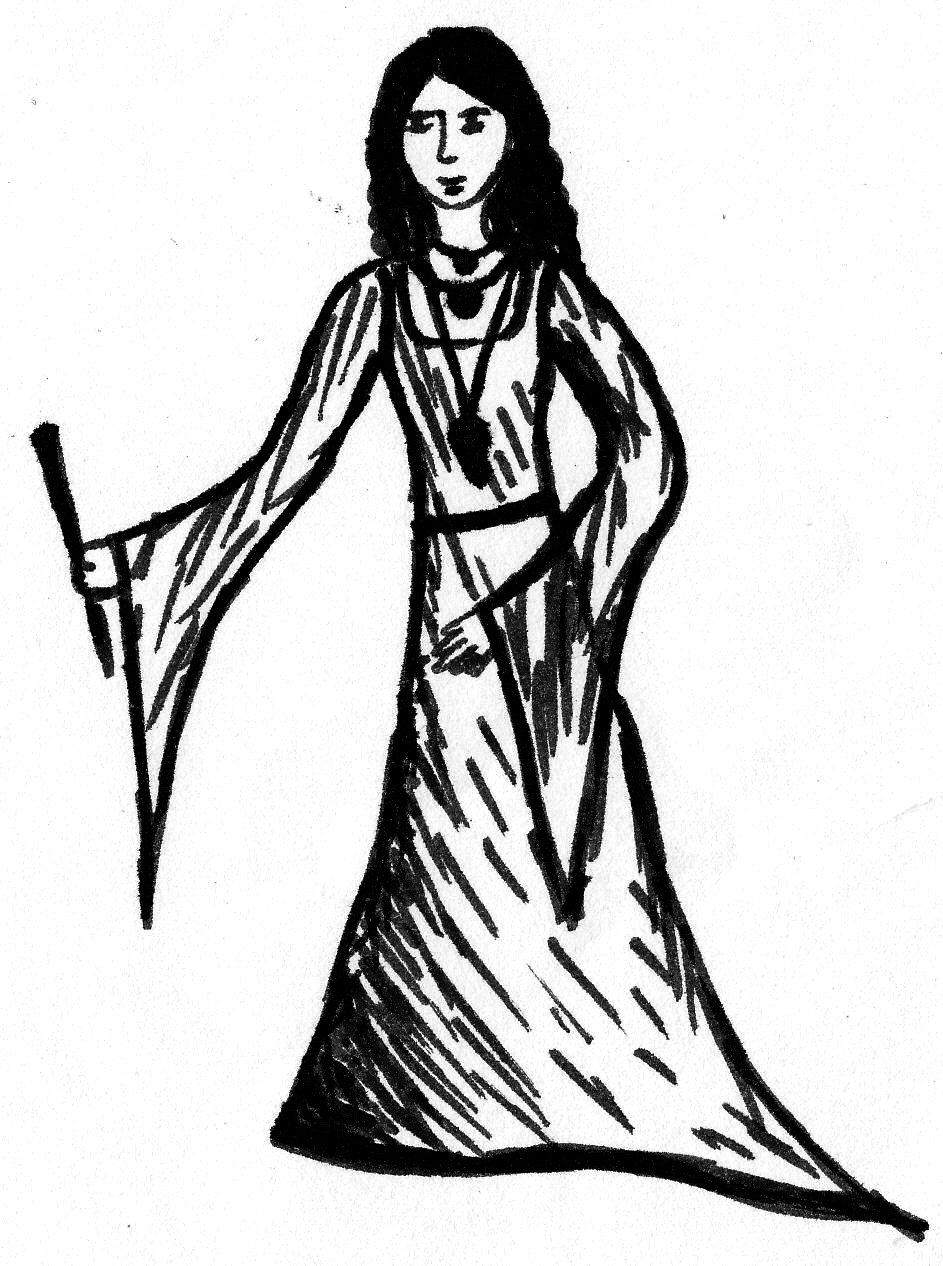
\includegraphics[width=5cm]{pict/carodejnice_z_amesbury}
\end{center}
\end{song}
\pagebreak

\begin{song}{Dál, dál, dál}{C}{Pacifik}
  \begin{SBVerse}
\Ch{C}{Za} horama zla\Ch{emi}{to} hoří v \Ch{F}{žilá}ch černejch \Ch{G}{skal},

\Ch{C}{hore}čkou tě\Ch{emi}{ }nohy pove\Ch{F}{do}--\Ch{G}{u. }

Ne\Ch{C}{pře}mejšlej chv\Ch{emi}{ilku} na to \Ch{F}{ruk}sak rychle \Ch{G}{sbal},

\Ch{F}{za}nech doma\Ch{D7}{ hol}ku zklama\Ch{G7}{nou}.
\end{SBVerse}
\begin{SBVerse}
Nezapomeň s sebou bibli nezbyde ti víc,

nežli v těžký chvíli modlení.

Eskymáci prej tam bydlej neroste tam nic,

prokleješ to zlatý kamení.

  \end{SBVerse}

\begin{SBChorus}
\Ch{C}{Dál} dál dál co \Ch{F}{ře}ka prame\Ch{C}{ní}
tam, kde břeh ukrejvá \Ch{D7}{dra}hý kamení.\Ch{G7}{   }
\Ch{C}{Dál} dál dál tou \Ch{F}{řek}ou máme\Ch{C}{ní},
tak kde na tě kejvá \Ch{G7}{zla}tý zname\Ch{C}{ní.}
\end{SBChorus}

\begin{SBVerse}
Snad se vrátíš jako tulák nebo jako pán,

nebo zůstaneš v tý zemi spát.

Nekoupíš si ani burák až se vrátíš k nám,

jak se budeš vo ty prachy bát.
\end{SBVerse}
\begin{SBVerse}
Holka se ti dávno vdala spadlo stavení,

na tebe už každej zapomněl.

Máma co se na tě smála už je pod zemí 

a pro ni si valoun zlata chtěl.
\end{SBVerse}

\begin{SBChorus}
\end{SBChorus}

\begin{SBVerse}
Postavíš si barák bílej v modrym pobřeží,

bankéři se vo tě budou prát.

Už nebudeš chlapče milej vo to neběží,

už nebudeš šťastnej nikde stát.
\end{SBVerse}

\begin{SBChorus}
\end{SBChorus}
\end{song}
\pagebreak

\setcounter{page}{18}
\begin{song}{Darmodej}{C}{Jaromír Nohavica}
  \begin{SBVerse}
\Ch{ami}{Šel} včera městem \Ch{emi}{muž} a šel po hlavní \Ch{ami}{třídě,} \Ch{emi}{ }

\Ch{ami}{šel} včera městem \Ch{emi}{muž} a já ho z okna \Ch{ami}{viděl}\Ch{emi}{, }

\Ch{C}{na} flétnu chorál \Ch{G}{hrá}l, znělo to jako \Ch{ami}{zvon}

a byl v tom všechen \Ch{emi}{žal,} ten krásný dlouhý \Ch{F}{tón,}

a já jsem náhle \Ch{F#dim}{věděl:} Ano, to je \Ch{E7}{on}, to je \Ch{ami}{on.}
\footnote{F\#dim lze nahradit D7}
  \end{SBVerse}
  \begin{SBVerse}
Vyběh' jsem do ulic jen v noční košili, 

v odpadcích z popelnic krysy se honily

a v teplých postelích lásky i nelásky 

tiše se vrtěly rodinné obrázky,

a já chtěl odpověď na svoje otázky, otázky.
  \end{SBVerse}
\begin{SBChorus}
$|$:\Ch{Ami}{Na,} nana\Ch{Emi}{na }nana\Ch{C}{na} nana \Ch{G}{nananána,}

\Ch{Ami}{na }nana\Ch{F}{na} nana\Ch{F#dim}{na nana} \Ch{E7}{nananána.} :$|$
\end{SBChorus}
\begin{SBVerse}
Dohnal jsem toho muže a chytl za kabát,

měl kabát z hadí kůže, šel z něho divný chlad,

a on se otočil, a oči plné vran,

a jizvy u očí, celý byl pobodán,

a já jsem náhle věděl kdo je onen pán onen pán

  \end{SBVerse}
\begin{SBVerse}

Celý se strachem chvěl,když jsem tak k němu došel,

a v ústech flétnu měl od Hieronyma Bosche,

stál měsíc nad domy jak čírka ve vodě,

jak moje svědomí, když zvrací v záchodě,

a já jsem náhle věděl: to je Darmoděj, můj Darmoděj.

  \end{SBVerse}
\begin{SBChorus}
Můj Darmoděj, vagabund osudů a lásek,

jenž prochází všemi sny,ale dnům vyhýbá se.

Můj Darmoděj, krásné zlo, jed má pod jazykem,

když prodává po domech jehly se slovníkem.

\end{SBChorus}
\begin{SBVerse}
Šel včera městem muž, podomní obchodník,

šel, ale nejde už, krev skápla na chodník,

já jeho flétnu vzal a zněla jako zvon

a byl v tom všechen žal, ten krásný dlouhý tón,

a já jsem náhle věděl: ano, já jsem on, já jsem:

  \end{SBVerse}
  
\begin{SBChorus}
Váš Darmoděj \dots
\end{SBChorus}
 \end{song}
\pagebreak

\input{song/a_desperát-II.tex}
\begin{song}{Divoké koně}{C}{Jaromír Nohavica}

\begin{SBVerse}

$|$: \Ch{ami}{Já }viděl \Ch{dmi}{divo}ké \Ch{ami}{koně}, \Ch{C}{běž}eli \Ch{dmi}{soum}ra\Ch{ami}{kem, }:$|$

\Ch{dmi}{Vzduch} \Ch{ami}{těžký} \Ch{dmi}{byl }a divně \Ch{ami}{voněl} \Ch{Ddmi}{tabá--}\Ch{F}{kem.}

\Ch{dmi}{Vzduch} \Ch{ami}{těžký} \Ch{dmi}{byl} a divně \Ch{ami}{voněl} \Ch{E7}{tabá}\Ch{ami}{kem}.

\end{SBVerse}

\begin{SBVerse}
$|$: Běželi, běžěli, bez uzdy a sedla, krajinou řek a hor, :$|$

$|$: Sper to čert, jaká touha je to vedla za obzor. :$|$
\end{SBVerse}

\begin{SBVerse}

$|$: Snad vesmír nad vesmírem, snad lístek na věčnost, :$|$

$|$: naše touho ještě neumírej, sil máme dost. :$|$

\end{SBVerse}

\begin{SBVerse}
$|$: V nozdrách sládne zápach klisen na břehu jezera, :$|$

$|$: milování je divoká píseň večera. :$|$
\end{SBVerse}

\begin{SBVerse}
$|$: Stébla trávy sklání hlavu , staví se do šiku, :$|$

$|$: král s dvořany přijíždí na popravu zbojníků. :$|$
\end{SBVerse}

\begin{SBVerse}
$|$: Chtěl bych jak divoký kůň běžet běžet, nemyslet na návrat, :$|$

$|$: s koňskými handlíři vyrazit dveře, to bych rád. :$|$
\end{SBVerse}

\begin{SBVerse}
Já viděl divoké koně\dots
\end{SBVerse}
\begin{center}
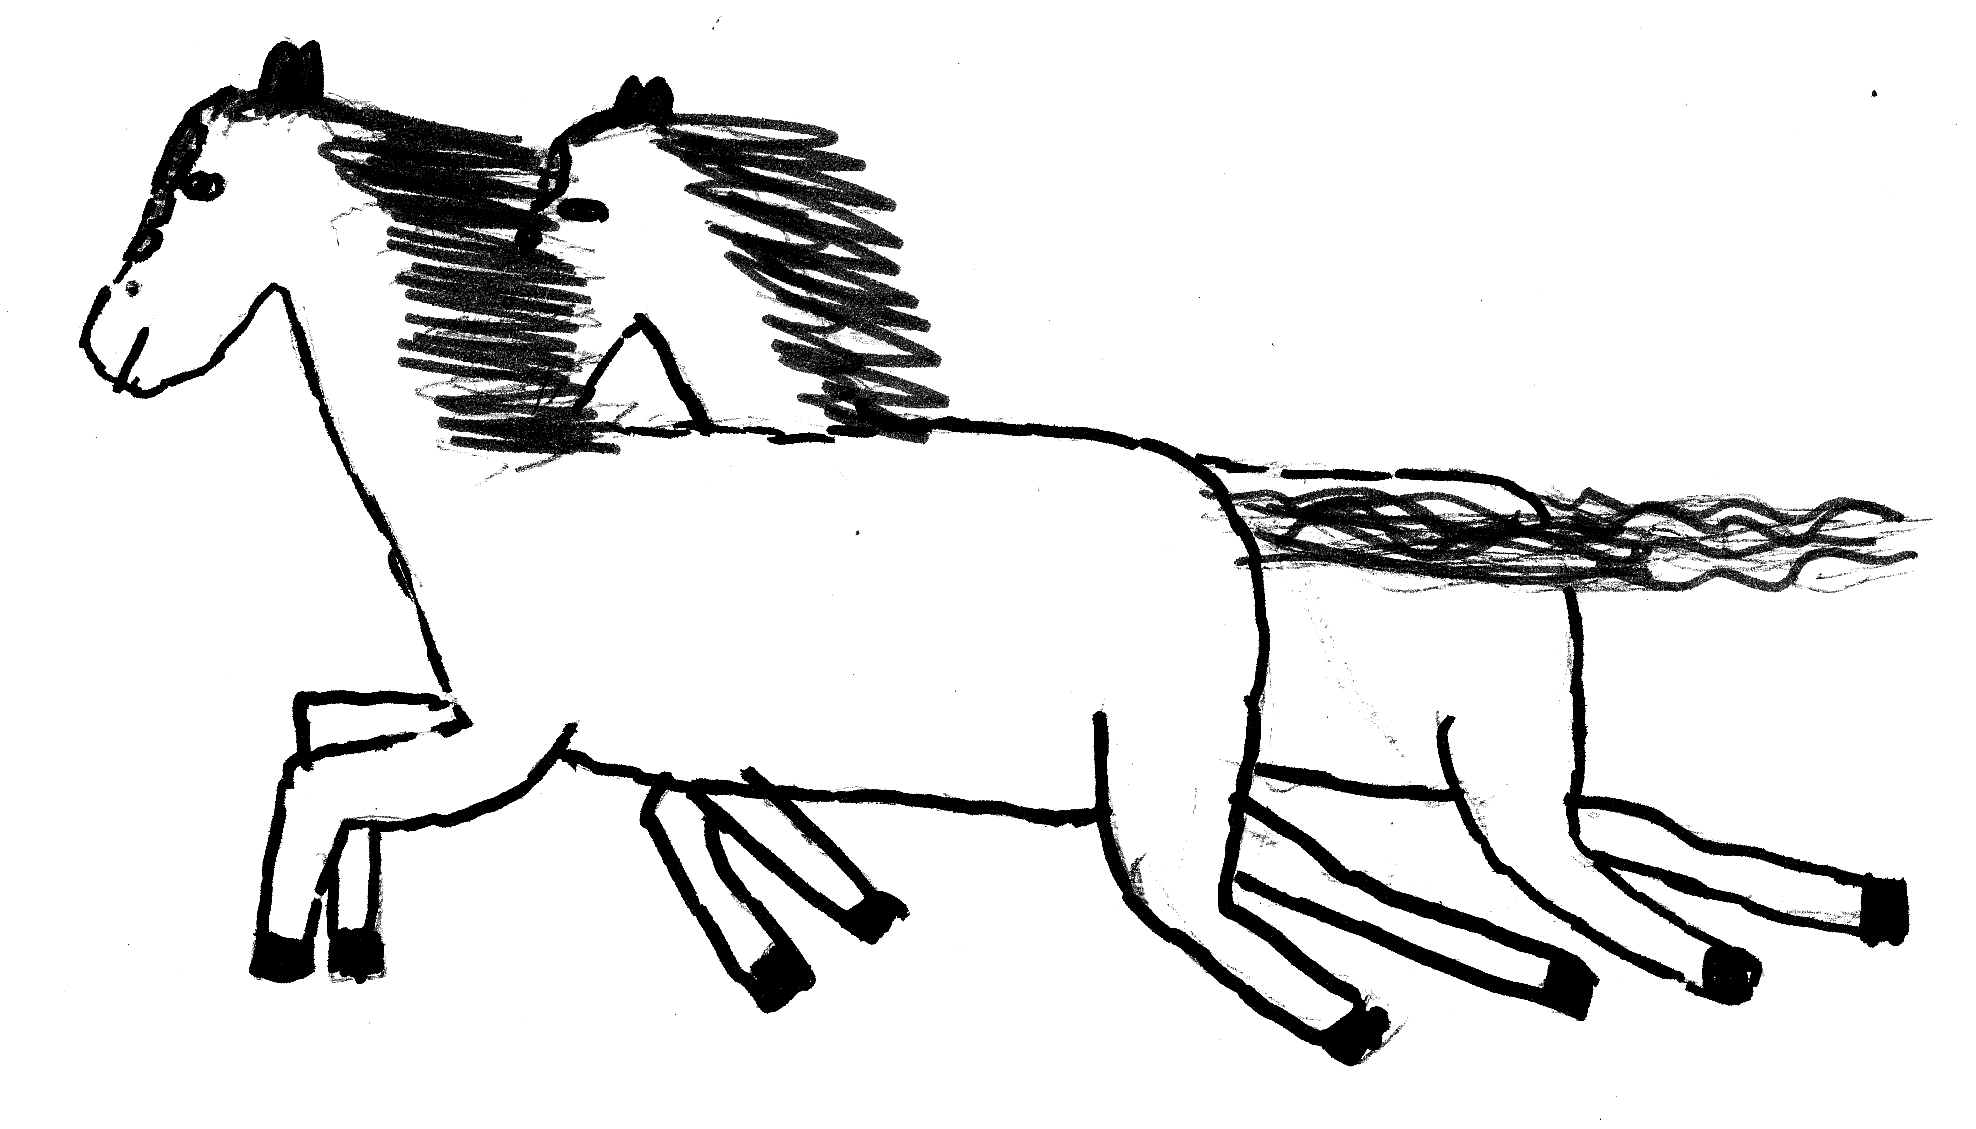
\includegraphics[width=5cm]{pict/divoci_kone}
\end{center}
\end{song}

\pagebreak
\setcounter{page}{23}
\begin{song}{Dva Havrani}{F}{Asonance}
\begin{SBVerse}

\Ch{dmi}{Když} jsem se z pole \Ch{C}{vrace}\Ch{dmi}{la,}

\Ch{dmi}{dva} havrany jsem \Ch{C}{slyše}\Ch{dmi}{la,}

\Ch{dmi}{jak} jeden \Ch{F}{druhého} se \Ch{C}{ptá:}

$|$: \Ch{dmi}{kdo} dneska veče\Ch{C}{ři} nám \Ch{dmi}{dá?} :$|$
\end{SBVerse}

\begin{SBVerse}
Ten první k druhému se otočil

a černým křídlem cestu naznačil,

krhavým zrakem k lesu hleděl

$|$: a takto jemu odpověděl. :$|$
\end{SBVerse}

\begin{SBVerse}
Za starým náspem, v trávě schoulený

tam leží rytíř v boji raněný,

a nikdo neví, že umírá,

$|$: jen jeho kůň a jeho milá. :$|$
\end{SBVerse}

\begin{SBVerse}
Jeho kůň dávno po lesích běhá

a jeho milá už jiného má,

už pro nás bude dosti místa,

$|$: hostina naše už se chystá. :$|$
\end{SBVerse}

\begin{SBVerse}
Na jeho bílé tváře usednem

a jeho modré oči vyklovem,

a až se masa nasytíme,

$|$: z vlasů si hnízdo postavíme. :$|$
\end{SBVerse}
\end{song}

\pagebreak

\begin{song}{Fi-li-mi}{As}{Spiritual kvintet}
\begin{SBVerse}
\Ch{fmi}{Čert} aby vzal už tuhle trať, kdo \Ch{G#}{hle}dáš práci, tak se strať,

že \Ch{fmi}{nemáš} prachy, no tak ať, jó, tak se \Ch{cmi}{na }to \Ch{fmi}{dívám.}


\end{SBVerse}
\begin{SBChorus}
\Ch{fmi}{Filimióri} júliei, \Ch{G#}{filimióri} júliei

\Ch{fmi}{filimióri} júliei,

vo tom \Ch{cmi}{si }teď \Ch{fmi}{zpí}vám
\end{SBChorus}
\begin{SBVerse}
Jen pražec chop a kolej suň, chyť lano táhni jako kůň, 

pod tíhou jako medveď fuň jó, tak se nato dívám !
\end{SBVerse}
\begin{SBVerse}
Z kůže se loupeš jako had, je vedro, že by jeden pad, 

na vodu smíš jen vzpomínat jó, tak se na to dívám !
\end{SBVerse}
\begin{SBVerse}
Když koněčně máš vody dost, určitě prěs ní stavíš most, 

kláda ti ráda zlomí kost jó, tak se nato dívám ! 

\end{SBVerse}
\begin{SBVerse}
Na rukách už jsem potěžkal většinu těch okolních skal, 

ještě to cejtí každej sval, jó tak se na to dívám.

\end{SBVerse}
\begin{SBVerse}
Slunce už dělá z trávy troud, jen kdybych se směl vocaď hnout

Na tuhle trať zapomenout, jó tak se na to dívam.
\end{SBVerse}
\begin{SBVerse}
Bůh mi víru zachovej a nasednout mi sílu dej

můj vagón bude pérovej jó o tom si teď zpívám.
\end{SBVerse}
\end{song}

\pagebreak
\input{song/a_frankie-dlouhán.tex}
\setcounter{page}{26}
\begin{song}{Hlídač krav}{C}{Jaromír Nohavica}
\begin{SBVerse}
\Ch{C}{Když} jsem byl malý, říkali mi naši:

Dobře se uč a jez chytrou kaši,

\Ch{F}{až} jednou vyrosteš, \Ch{G}{budeš} doktorem \Ch{C}{práv}.

Takový doktor si sedí pěkně v suchu,

bere velký peníze a škrábe se v uchu,

\Ch{F}{já} jim ale na to řek': Ch\Ch{G}{ci} být hlídačem \Ch{C}{krav.}
\end{SBVerse}
\begin{SBChorus}
Já chci \Ch{C}{mít} čapku s bambulí nahoře,

jíst kaštany a mýt se v lavoře,

\Ch{F}{od} rána po celý \Ch{G}{den} zpívat si \Ch{C}{jen,}

zpívat si: \Ch{C}{pam} pam pam\Ch{F}{ } \Ch{G}{\dots} \Ch{C}{ } 
\end{SBChorus}
\begin{SBVerse}
K vánocům mi kupovali hromady knih,

co jsem ale vědět chtěl, to nevyčet' jsem z nich:

nikde jsem se nedozvěděl, jak se hlídají krávy.

Ptal jsem se starších a ptal jsem se všech,

každý na mě hleděl jako na pytel blech,

každý se mě opatrně tázal na moje zdraví.
\end{SBVerse}
\begin{SBVerse}
Dnes už jsem starší a vím, co vím,

mnohé věci nemůžu a mnohé smím,

a když je mi velmi smutno, lehnu si do mokré trávy.

S nohama křížem a s rukama za hlavou

koukám nahoru na oblohu modravou,

kde se mezi mraky honí moje strakaté krávy.
\end{SBVerse}
\end{song}

\pagebreak

\begin{song}{Hospoda U Davida}{G}{Fleret}
\begin{SBVerse}
V \Ch{C}{hospodě} \Ch{G}{na} náměs\Ch{C}{tí} může\Ch{G}{te} při troše \Ch{ami}{štěs}tí

sehnat \Ch{D}{místo} u sto\Ch{G}{lu,}

sednout si na lavi\Ch{C}{ci,} dát si \Ch{G}{pravou} kyseli\Ch{ami}{ci}

anebo \Ch{D}{rum} a kofo\Ch{G}{lu}.

Říká se tam "U Davida", klasická třetí třída,

zákaz her s výjimkou domina,

a když je někdy pod psa venku, 

hospodský též dá si sklenku,

přisedne \Ch{D}{k }vám \Ch{G}{a }vzpomí\Ch{C}{ná}.
\end{SBVerse}
\begin{SBChorus}
\Ch{H}{Ač} je to téměř k nevíře, já \Ch{emi}{býval} slavným kumštýřem,

\Ch{H}{zpíval} a napříč flétnou \Ch{emi}{hrál},

\Ch{H}{procestoval} kraje cizí, v \Ch{emi}{rozhlase} a v \Ch{A}{televizi}

\Ch{C}{každej} mě \Ch{D}{znal},

\Ch{H}{a }holky krásný jako břízky \Ch{emi}{nosily} mi z domu řízky,

\Ch{H}{po }koncertě rovnou do šat\Ch{emi}{ny, }

\Ch{H}{za }podpisy do cancáku \Ch{emi}{vlezly} mi až \Ch{A}{do} spacáku,

\Ch{C}{ale }to je \Ch{D}{dnes} už neplat\Ch{G}{ný.}
\end{SBChorus}

\begin{SBVerse}
Pak se napije a kývá hlavou, jako by přemýšlel nad zašlou slávou,

a je ticho a jen pendlovky jdou,

pak vstane a jde za své pípy, a za chvíli už zas vtipy

rozléhají se hospodou.

A když nese další várku jak Děda Mráz s nůší dárků,

štamgastům se oči rozzáří,

co tam po odjezdu vlaků, hned si dají po panáku,

tržba se dnes jistě vydaří.
\end{SBVerse}
\begin{SBChorus}
Jó, je to dnes až k nevíře, ten chlap býval slavným kumštýřem,

zpíval a napříč flétnou hrál,

procestoval kraje cizí, v rozhlase a v televizi

každej ho znal,

A teď tady pivo točí a dojetím mu vlhnou oči,

když sem přijdou kluci s kytarou,

stojí v teskném zamyšlení a hosté mizí bez placení

a říkají si, že je zas pod párou.
\end{SBChorus}
\begin{SBVerse}
Až někdy navštívíte Vizovice, zaparkujte u silnice,

tož tam, co je tech nejvíc obchodů,

rozhlédněte se vpředu, vzadu, a, nemáte-li oční vadu,

ucítíte hospodu.

A když se zeptáte na hospodského, dovíte se od každého,

že je to notorický lhář, ale já ho \Ch{C}{viděl} jednou v \Ch{G/H}{květnu,}

jak tam \Ch{ami}{stál} a v ruce \Ch{D}{flétnu,} a kolem \Ch{G}{hlavy}, 

kolem hlavy vám měl svato\Ch{C}{zář.}
\end{SBVerse}
\end{song}

\pagebreak
\begin{song}{Hrobař}{G}{Premier}

\begin{SBVerse}

V \Ch{G}{mládí} jsem se učil hrobařem

\Ch{emi}{jezdit} s hlínou, jezdit s trakařem

\Ch{C}{kopat} hroby byl můj ide\Ch{D}{ál}.

\end{SBVerse}

\begin{SBVerse}

Jezdit s hlínou, jezdit s vozíkem

s černou rakví, bílým pomníkem

toho bych se nikdy nenadál.

\end{SBVerse}

\begin{SBVerse}

Že do módy příjde kremace

černej hrobař bude bez práce

toho bych se nikdy nenadál nenadál.

\end{SBVerse}

\begin{SBVerse}

Kolem projel vůz milionáře

záblesk světel pad mi do tváře,

marně skřípěj kola brzdící.

\end{SBVerse}

\begin{SBVerse}

Stoupám vzhůru stoupám ke hvězdám

tam se s černou rakví neshledám,

sbohem bílé město zářící.



Sbohem moje mesto

vzpominat budu presto

jak jsem poznal tvůj smich a tvůj pláč 

\end{SBVerse}

\begin{SBVerse}

Na na na .......

\end{SBVerse}

\end{song}

\pagebreak
\todo{TODO:additional verses}
\begin{song}{Hučka}{G}{Zelenáči}
\begin{SBVerse}
Hučku \Ch{G}{svou} na pozdrav smekám, světla \Ch{ami}{vlaků} vidím plát,

tak na \Ch{D}{svůj} nárazník čekám, už jsem \Ch{C}{tě} měl ako\Ch{G}{rát.}

Zejtra ráno, až se vzbudíš, zjistíš, že se slehla zem

a tvůj miláček že pláchnul půlnočním expresem.
\end{SBVerse}
\begin{SBChorus}
Za chví li už budu v dáli, za chví li mi bude fajn,

o tvý  lásce, která pálí, nebu du mít ani  šajn.

Za chví li už budu v dáli, za chví li mi bude fajn,

o tvý  lásce, která pálí, nebu du mít ani  šajn.
\end{SBChorus}
\begin{SBVerse}
Nejdřív zní vlakovej zvonec, pak píšťala, je mi hej,

konečně vím, že je konec naší lásce tutovej.

Z kapsy tahám harmoniku, tuláckej son budu hrát,

sedím si na nárazníku a je mi tak akorát. 
\end{SBVerse}
\end{song}

\pagebreak
{
\begin{song}{Hudsonský šífy}{C}{Wabi Daněk}
\begin{SBVerse}
Ten kdo \Ch{ami}{nezná} hukot vody lopatkama\Ch{C}{ vířený},

jako \Ch{G}{já,} jako \Ch{ami}{já}.

Kdo hudsonský slapy nezná sírou \Ch{G}{pekla} sířený,
 
ať se \Ch{ami}{na }hudsonský \Ch{G}{šífy} najmout \Ch{ami}{dá,} \Ch{G}{jo} \Ch{G#}{ho} \Ch{ami}{ho}.
\end{SBVerse}
\begin{SBVerse}
Ten kdo nepřekládal uhlí, šíf když na mělčinu vjel, 

málo zná, málo zná.

Ten kdo neměl tělo ztuhlý až se nočním chladem chvěl,

ať se na hudsonský šífy najmout dá, jo ho ho.

\end{SBVerse}
\begin{SBChorus}
Tak \Ch{F}{ahoj}, páru tam \Ch{ami}{hoď}, ať \Ch{G}{do} pekla se dřívě \Ch{ami}{dohra}bem

\Ch{G}{Jo} \Ch{G#}{ho }\Ch{ami}{ho, }\Ch{G}{jo} \Ch{G#}{ho }\Ch{ami}{ho.}
\end{SBChorus}
\begin{SBVerse}

Ten kdo nezná noční zpěvy zarostlenejch lodníků,

jako já, jako já.

Ten kdo cejtí se bejt chlapem, umí dělat rotyku,

ať se na hudsonský šífy najmout dá, jo ho ho.

Ten kdo má na bradě mlíko,kdo se rumem neopil, 

málo zná, málo zná.

Kdo necejtil hrůzu z vody, kde se málem utopil,

ať se na hudsonský šífy najmout dá, jo ho ho.
\end{SBVerse}
\begin{SBVerse}
Kdo má roztrhaný boty, kdo má pořád jenom hlad, 

jako já, jako já.

Kdo chce celý noci čuchat pekelního ohně smrad, 

ať se na hudsonský šífy najmout dá, jo ho ho. 

Kdo chce zhebnout třeba zejtra, komu je to všechno fuk,

kdo je sám, jako já.

Kdo má srdce v správným místě, kdo je prostě prima kluk,

ať se na hudsonský šífy najmout dá, jo ho ho.
\end{SBVerse}
\end{song}






\pagebreak
\setcounter{page}{35}
\begin{song}{Jarní tání}{C}{Jan Nedvěd}

\begin{SBVerse}

Když první \Ch{ami}{tání} \Ch{dmi}{cestu} sněhu \Ch{C}{zkříží}\Ch{F}{}

a nad le\Ch{dmi}{dem} se \Ch{E}{voda} obje\Ch{ami}{ví.}

Voňavá \Ch{ami}{zem} se \Ch{dmi}{sněhem} tiše \Ch{C}{plíží}\Ch{F}{}

tak nějak \Ch{dmi}{líp }si \Ch{E}{balím,} proč bůh\Ch{ami}{ví.}

\end{SBVerse}

\begin{SBChorus}

Přišel čas \Ch{F}{slunce,} zrození a \Ch{C}{tratí}

na kterejch \Ch{F}{potkáš} kluky ze všech \Ch{C}{stran}\Ch{E7}{}

$|$: Hubenej \Ch{ami}{Joe,} Čára, Ušoun se ti \Ch{dmi}{vrát}í,

oživne \Ch{F}{kemp}, \Ch{E}{jaro} vítej k \Ch{ami}{nám}.\Ch{E7}{ :$|$}

\end{SBChorus}

\begin{SBVerse}

Kdo ví jak voní země, když se budí

pocit má vždy jak zrodil by se sám.

Jaro je lék na řeči, co nás nudí

na lidi, co chtěj zkazit život nám.

\end{SBVerse}

\begin{SBVerse}

Zmrznout by měla, kéž by se tak stalo

srdce těch pánů, co je jim vše fuk.

Pak bych měl naději, že i příští jaro

bude má země zdravá jako buk.

\end{SBVerse}

\end{song}

\pagebreak

\begin{song}{Jaro}{C}{}

\begin{SBVerse}

\Ch{ami}{My }čekali \Ch{C}{jaro,} a \Ch{G}{zatím} přišel \Ch{ami}{mráz,}

\Ch{ami}{tak }strašlivou \Ch{C}{zimu,} ne\Ch{G}{zažil} nikdo z \Ch{ami}{nás.}

\Ch{ami}{Z těžk}ých černých \Ch{C}{mraků} se \Ch{G}{stále} sypal \Ch{ami}{sníh}

\Ch{ami}{a ván}ice \Ch{C}{sílí} v po\Ch{G}{ryvech} ledo\Ch{ami}{vých.}

Z \Ch{C}{chýší} dřevo mizí a \Ch{G}{mouky} ubývá,

\Ch{dmi}{do }sýpek se raději už \Ch{G}{nikdo} nedívá.

\Ch{C}{Zvěř} z okolních lesů nám \Ch{G}{stála} u dveří

\Ch{dmi}{a hla}doví ptáci při\Ch{G}{lét}li za zvěří, a stále \Ch{ami}{blíž.}

\end{SBVerse}

\begin{SBVerse}

Pak jednoho dne večer, to už jsem skoro spal.

Když vystrašený soused na okno zaklepal.

Můj chlapec doma leží, v horečkách vyvádí.

Já do města bych zajel, doktor snad poradí.

Půjčil jsem mu koně, a když sedlo zapínal,

dříve, než se rozjel, jsem ho ještě varoval:

Nejezdi naší zkratkou, je tam příkrej sráz,

a v téhleté bouři tam snadno zlámeš vaz, tak neriskuj.

\end{SBVerse}

\begin{SBVerse}

Na to chmurné ráno, dnes nerad vzpomínám.

Na tu hroznou chvíli, když kůň se vrátil sám.

Trvalo to dlouho, než se vítr utišil.

Na sněhové pláně si každý pospíšil.

Jeli jsme tou zkratkou, až k místu, které znám,

kterým bych té noci nejel ani sám.

Pak ho někdo spatřil, jak leží pod srázem.

Krev nám tuhla v žilách nad tím obrazem, já kloubouk sňal.

\end{SBVerse}

\begin{SBVerse}

Někdy, ten kdo spěchá se domů nevrací...
\end{SBVerse}
\end{song}

\pagebreak
\input{song/a_jasný-jak-facka.tex}
\begin{song}{Jdou po mě jdou}{D}{Jaromír Novavica}

\begin{SBVerse}

Býval jsem \Ch{D}{chudý} jak \Ch{G}{kostelní} \Ch{D}{myš,}

na půdě \Ch{f#mi}{půdy} jsem \Ch{hmi}{míval} svou \Ch{A}{skrýš,}

$|$: \Ch{G}{pak} jednou v \Ch{D}{létě} \Ch{A}{řek'} jsem si: \Ch{D}{bať,}

svět fackuje tě, a \Ch{G}{tak} mu to \Ch{D}{vrať.} :$|$
\end{SBVerse}
\begin{SBVerse}
Když mi dát nechceš, já vezmu si sám,

zámek jde lehce a adresu znám,

$|$: zlato jak zlato, dolar či frank,

tak jsem šel na to do National Bank. :$|$
\end{SBVerse}

\begin{SBChorus}

Jdou po mně, \Ch{D}{jdou,} \Ch{G}{jdou,} \Ch{D}{jdou,}

na každém \Ch{f#mi}{rohu} ma\Ch{hmi}{jí} fotku \Ch{A}{mou,}

\Ch{G}{kdyby} mě \Ch{D}{chytli,} \Ch{A}{jó,} byl by \Ch{D}{ring,}

\Ch{G}{tma} jako v \Ch{D}{pytli} je v \Ch{C}{celách} Sing-\Ch{G}{sing.}\Ch{A}{} \Ch{D}{}

\end{SBChorus}

\begin{SBVerse}

Ve státě Iowa byl od poldů klid,

chudičká vdova mi nabídla byt,

$|$: jó, byla to kráska, já měl peníze,

tak začla láska jak z televize. :$|$
\end{SBVerse}
\begin{SBVerse}
Však půl roku nato řekla mi:"Dost,

tobě došlo zlato, mně trpělivost,

$|$: sbal svých pár švestek a běž si, kam chceš,"

tak jsem na cestě a chudý jak veš. :$|$

\end{SBVerse}

\begin{SBChorus}

\end{SBChorus}
\begin{SBVerse}
Teď ve státě Utah žiju spokojen,

pípu jsem utáh' a straním se žen,

$|$: jó, kladou mi pasti a do pastí špek,

já na ně mastím, jen ať mají vztek. :$|$

\end{SBVerse}

\begin{SBChorus}

Jdou po mně jdou, jdou, jdou,

na nočních stolcích mají fotku mou,

kdyby mě klofly, jó, byl by ring,

být pod pantoflí je hůř než v Sing-sing.

\end{SBChorus}

\end{song}

\pagebreak
\begin{song}{Když mě brali za vojáka}{C}{Jaromír Nohavica}

\begin{SBVerse}

\Ch{ami}{Když} mě brali za vo\Ch{C}{jáka,} \Ch{G}{stříhali} mě doho\Ch{C}{la,}

\Ch{dmi}{vypadal} jsem jako \Ch{ami}{blbec}, \Ch{E}{jak} ti všichni doko\Ch{F}{la,}

\Ch{G}{la,} \Ch{C}{la,} \Ch{G}{la,} \Ch{ami}{jak} ti všichni \Ch{E}{doko}\Ch{ami}{la.}

\end{SBVerse}

\begin{SBVerse}

Zavřeli mě do kasáren začali mě učiti,

jak mám správný voják býti a svou zemi chrániti.

\end{SBVerse}

\begin{SBVerse}

Na pokoji po večerce ke zdi jsem se přitulil.

Vzpomněl jsem si na svou milou, krásně jsem si zabulil.

\end{SBVerse}

\begin{SBVerse}

Když přijela po půl roce, měl jsem zrovna zápal plic,

po chodbě furt někdo chodil, tak nebylo z toho nic.

\end{SBVerse}

\begin{SBVerse}

Neplačte, vy oči moje, ona za to nemohla,

protože mladá holka lásku potřebuje,

a tak si k lásce pomohla.

\end{SBVerse}

\begin{SBVerse}

Major nosí velkou hvězdu, před branou ho potkala.

Řek jí, že má zrovna volný kvartýr, tak se sbalit nechala.

\end{SBVerse}

\begin{SBVerse}

Co je komu do vojáka, když ho holka zradila,

na shledanou, pane Fráňo Šrámku, písnička už skončila,

la, la, la, jakpak se Vám líbila?

la, la, la; no, nic moc extra nebyla\dots

\end{SBVerse}

\end{song}

\pagebreak
\begin{song}{Kluziště}{C}{Karel Plíhal}

\begin{SBVerse}

\Ch{C}{Strejček} \Ch{emi7}{kovář} c\Ch{ami7}{hytil} k\Ch{C}{leště,} \Ch{Fmaj7}{uštíp'} z \Ch{C}{noční}\Ch{Fmaj7}{ oblo--}\Ch{G}{hy}

   \Ch{C}{jednu} m\Ch{emi7}{alou} ka\Ch{ami7}{pku d}\Ch{C}{eště,} t\Ch{Fmaj7}{a mu} sp\Ch{C}{adla} p\Ch{Fmaj7}{od noh}\Ch{G}{y,}

   \Ch{C}{nejdřív }\Ch{emi7}{ale }chy\Ch{ami7}{til sl}\Ch{C}{inu, t}\Ch{Fmaj7}{ak šáh' k}\Ch{C}{amsi} \Ch{Fmaj7}{pro pi}vo\Ch{G}{,}

   \Ch{C}{pak při}\Ch{emi7}{táhl} \Ch{ami7}{kovad}\Ch{C}{linu}\Ch{Fmaj7}{ a} \Ch{C}{obrovský} \Ch{Fmaj7}{kladi--}\Ch{G}{vo.}

\end{SBVerse}

\begin{SBChorus}

   Zatím t\Ch{C}{ři }bílé v\Ch{emi7}{rány }pě\Ch{ami7}{kně za} se\Ch{C}{bou}

   kolem jd\Ch{Fmaj7}{ou,} někam jd\Ch{C}{ou,} do rytm\Ch{D7}{u se} kývaj\Ch{G}{í,}

   tyhle tř\Ch{C}{i bílé} vr\Ch{emi7}{ány }pě\Ch{ami7}{kně za} seb\Ch{C}{ou}

   kolem jd\Ch{Fmaj7}{ou, někam} jd\Ch{C}{ou, nedojd}\Ch{Fmaj7}{ou, ne}dojd\Ch{C}{ou.}

  \end{SBChorus}

\begin{SBVerse}

   Vydal z hrdla mocný pokřik ztichlým letním večerem,

   pak tu kapku všude rozstřík' jedním mocným úderem,

   celej svět byl náhle v kapce a vysoko nad námi

   na obrovské mucholapce visí nebe s hvězdami.

\end{SBVerse}

\begin{SBVerse}

   Zpod víček mi vytrysk' pramen na zmačkané polštáře,

   kdosi mě vzal kolem ramen a políbil na tváře,

   kdesi v dálce rozmazaně strejda kovář odchází,

   do kalhot si čistí ruce umazané od sazí.

 \end{SBVerse}

 \end{song} 

\pagebreak
\begin{song}{Kometa}{C}{Jaromír Nohavica}

\begin{SBVerse}

\Ch{ami}{Spatřil} jsem kometu, oblohou letěla,

chtěl jsem jí zazpívat, ona mi zmizela,

\Ch{dmi}{zmizela} jako laň \Ch{G7}{u lesa} v remízku,

\Ch{C}{v }očích mi zbylo jen \Ch{E7}{pár} žlutých penízků.

\end{SBVerse}

\begin{SBVerse}

Penízky ukryl jsem do hlíny pod dubem,

až příště přiletí, my už tu nebudem,

my už tu nebudem, ach, pýcho marnivá,

spatřil jsem kometu, chtěl jsem jí zazpívat.

\end{SBVerse}

\begin{SBChorus}

\Ch{ami}{O vodě}, o trávě, \Ch{dmi}{o lese,} \Ch{G7}{o }smrti, se kterou smířit \Ch{C}{nejde} se,

\Ch{ami}{o }lásce, o zradě, \Ch{dmi}{o svě}tě

\Ch{E}{a o }všech lidech, co kdy \Ch{E7}{žili} na téhle \Ch{ami}{planetě.}

\end{SBChorus}

\begin{SBVerse}

Na hvězdném nádraží cinkají vagóny,

pan Kepler rozepsal nebeské zákony,

hledal, až nalezl v hvězdářských triedrech

tajemství, která teď neseme na bedrech.

\end{SBVerse}

\begin{SBVerse}

Velká a odvěká tajemství přírody,

že jenom z člověka člověk se narodí,

že kořen s větvemi ve strom se spojuje

a krev našich nadějí vesmírem putuje.

\end{SBVerse}

\begin{SBChorus}

Na na na ...

\end{SBChorus}

\begin{SBVerse}

Spatřil jsem kometu, byla jak reliéf

zpod rukou umělce, který už nežije,

šplhal jsem do nebe, chtěl jsem ji osahat,

marnost mne vysvlékla celého donaha.

\end{SBVerse}

\begin{SBVerse}

Jak socha Davida z bílého mramoru

stál jsem a hleděl jsem, hleděl jsem nahoru,

až příště přiletí, ach, pýcho marnivá,

my už tu nebudem, ale jiný jí zazpívá.

\end{SBVerse}

\begin{SBChorus}

O vodě, o trávě, o lese, o smrti, se kterou smířit nejde se,

o lásce, o zradě, o světě, bude to písnička o nás a kometě.

\end{SBChorus}

\end{song}

\pagebreak
\setcounter{page}{44}
\begin{song}{Kozel}{G}{Jaromír Nohavica}

\begin{SBVerse}

Byl jeden \Ch{G}{pán }ten kozla \Ch{C}{měl}

velice \Ch{D7}{si} s ním rozu\Ch{G}{měl}

Měl ho moc rád, opravdu \Ch{C}{moc}.

Hladil mu \Ch{D7}{fous} na dobrou \Ch{G}{noc}\Ch{D7}{} \Ch{G}{}
\end{SBVerse}
\begin{SBVerse}
Jednoho dne se kozel splet

rudé tričko pánovi sněd

Když to pán zřel, zařval jejé

Svázal kozla na koleje
\end{SBVerse}
\begin{SBVerse}
Zapískal vlak, kozel se lek

To je má smrt, mečel mek mek

Jak tak mečel, vykašlal pak

Rudé tričko, čímž stopnul vlak.
\end{SBVerse}
\end{song}

\pagebreak

 \begin{song}{Lord Willoughby}{C}{Asonance}
\begin{SBVerse}
 Byl \Ch{ami}{pat}náctý den \Ch{G}{lé}\Ch{C}{ta} a \Ch{F}{hor}ký vítr \Ch{E}{vál}, když 

   \Ch{ami}{u Fl}ander Lord \Ch{G}{Will}ough\Ch{C}{by} s ang\Ch{F}{lic}kým vojskem \Ch{E}{stál},
   
   
   od \Ch{F}{ostří} mečů \Ch{C}{bly}štivých se slunce od\Ch{F}{rá}\Ch{G}{ží,} 

   když \Ch{C}{do} rozhodné \Ch{ami}{bitvy} jeho \Ch{F}{vojsko} \Ch{E}{vy}rá\Ch{ami}{ží.} 
\end{SBVerse}
\begin{SBVerse}
Nejlepší muži Anglie za královnu jdou se bít, 

   však nejchrabřejší z chrabrých je sám Lord Willoughby, 

   Čtyřicet tisíc mužů sem španělský král vzal, 

   by potupnou porážku Anglii přichystal. 
\end{SBVerse}
\begin{SBVerse}
Už sedm hodin dlouhých řev bitvy burácí 

   a síly našich mužů se zvolna vytrácí, 

   vojáci už i z louží začali vodu pít, 

   když v tom strašlivém horku jinou nemohli mít. 
\end{SBVerse}
\begin{SBVerse}
Zní svistot ostrých šípů i koule létají 

   a angličtí vojáci po stovkách padají 

   a o jejich porážce už není pochyby, 

   když do útoku troubí statečný Willoughby. 
\end{SBVerse}
\begin{SBVerse}
Do znavených vojáků on novou sílu vlil, 

   na španělské oddíly tak tvrdě udeřil, 

   že španělská armáda útoku podléhá 

   a vítězné volání se vůkol rozléhá. 
\end{SBVerse}
\begin{SBVerse}
Tak slyšte všichni věrní, když Bůh nám pomáhá, 

   i s přesilou nepřátel Anglie vyhrává, 

   tak jako tam u Flander za španělské palby, 

   kde zvítězit dokázal slavný Lord Willoughby.
   \end{SBVerse}
   \end{song}

\pagebreak
\begin{song}{Marsyas a Apollon}{G}{}

\begin{SBVerse}

\Ch{G}{Ta} krásná dívka, \Ch{ami}{co} se bojí o \Ch{D}{svoji} krásu

\Ch{G}{Athéna} \Ch{emi}{jméno} má \Ch{C}{za} starých \Ch{G}{dávných} časů

\Ch{G}{odhodí} flétnu, \Ch{ami}{hrát} nejde s \Ch{D}{nehybnou} tváří

\Ch{G}{kdo} si ji \Ch{emi}{najde} dřív, \Ch{C}{tomu} se \Ch{G}{přání} zmaří.

\end{SBVerse}

\begin{SBChorus}

\Ch{emi}{Tak }si Marsyas \Ch{D}{mámen} flétnou \Ch{emi}{věří,} že \Ch{C}{musí} přetnout

$|$: \Ch{G}{jedno} pravidlo, \Ch{D}{sázku} a \Ch{C}{hrát} \Ch{G}{líp} \Ch{D}{než} \Ch{G}{bůh} :$|$

\end{SBChorus}

\begin{SBVerse}

Bláznivý nápad, snad nejvýš Marsyas míří

Apollón souhlasí, oba se s trestem smíří

král Midas má říct, kdo je lepši, Apollón zpívá

o život soupeří, jen jeden vítěz bývá

\end{SBVerse}

\begin{SBChorus}

Tak si Marsyas mámen flétnou věří a musí přetnout

$|$: jedno pravidlo, sázku a hrát líp než bůh :$|$

\end{SBChorus}

\begin{SBVerse}

Obrátí nástroj, už ví, že nebude chválen

prohrál a zápolí podveden vůlí krále

sám v tichém hloučku, sám na strom připraví ráhno

satyra k hrůze všech zaživa z kůže stáhnou

\end{SBVerse}

\begin{SBChorus}

Tak si Apollón změřil síly, každý se musel mýlit

$|$: Nikdo nemůže kouzlit a hrát líp než bůh :$|$

\end{SBChorus}

\begin{SBVerse}

Ta krásná dívka, co se bála o svoji krásu

dárkyně moudrosti za starých dávných časů

Teď v tichém hloučku, v jejích rukou úroda, spása

Athéna jméno má, chybí jí tvář a krása

\end{SBVerse}

\begin{SBChorus}

Dy dy dy \dots

\end{SBChorus}

\end{song}

\pagebreak
\begin{song}{Mezi horami}{C}{Čechomor}

\begin{SBVerse}

$|$: \Ch{ami}{Mezi} \Ch{G}{hora}\Ch{ami}{mi}, \Ch{ami}{lipka} \Ch{G}{ze}le\Ch{ami}{ná} :$|$

$|$: \Ch{C}{zabili} Janka \Ch{G}{Janíčka,} \Ch{ami}{Janka} \Ch{ami}{miesto} \Ch{G}{je}le\Ch{ami}{ňa :}$|$

\end{SBVerse}

\begin{SBVerse}



Keď ho zabili zamordovali,

na jeho hrobě, na jeho hrobě, kříž postavili,

\end{SBVerse}

\begin{SBVerse}

Ej, křížu, křížu, ukřižovaný

zde leží Janík, Janíček, Janík, zamordovaný.

\end{SBVerse}

\begin{SBVerse}

Tu šla Anička, plakat Janíčka,

hned na hrob padla, a viac něvstala, dobrá Anička.

\end{SBVerse}

\end{song}

\pagebreak
\begin{song}{Morituri te salutant}{C}{Karel Kryl}
\begin{SBVerse}
Cesta je \Ch{ami}{prach} a \Ch{G}{šterk} a \Ch{dmi}{udusaná} \Ch{ami}{hlína} 

a šedé \Ch{F}{šmrouhy }\Ch{G7}{kreslí} do vla\Ch{C}{sů}

$|$: a z hvězdných \Ch{dmi}{drah} má \Ch{G}{šperk} co \Ch{C}{kamením} se \Ch{ami}{spíná}

a pírka \Ch{G}{tou}hy z křídel pega\Ch{ami}{sů. }:$|$\Ch{ami}{} \Ch{G}{} \Ch{ami}{} \Ch{E7}{}

\end{SBVerse}
\begin{SBVerse}

Cesta je bič, je zlá jak pouliční dáma, 

má v ruce štítky a pase staniol, 

$|$: a z očí chvíč jí plá, když háže do neznáma, 

dvě křehké snítky rudých gladiol.:$|$\Ch{ami}{}


\end{SBVerse}
\begin{SBChorus}
Seržante \Ch{G}{písek} je bílý jak paže Daniely,

\Ch{ami}{počkejte} chvíli mé oči uviděli,

\Ch{G}{tu} strašne dávnou vteřinu zapomnění,

\Ch{ami}{Seržante} mávnou \Ch{G7}{a bud}em zasvěceni,

\Ch{ami}{Mor}ituri te salutant,\Ch{E}{mor}ituri te salutant.\Ch{ami}{} \Ch{G}{} \Ch{ami}{} \Ch{E7}{}
\end{SBChorus}
\begin{SBVerse}
Tou cestou dál jsem šel, kde na zemi se zmítá,

a písek víří křídla holubí 

a marš mi hrál zvuk děl co uklidnění skrýtá,

a zvedá chmýři které zahubí.
\end{SBVerse}
\begin{SBVerse}
Cesta je tér a prach a udusaná hlína,

mosazná včelka od vlkodlaka,

rezavý kvér, můj prach a sto let stará špína,

a děsně velká bíla oblaka.
\end{SBVerse}
\end{song}

\pagebreak
\setcounter{page}{55}
\begin{song}{Mumie}{C}{Slávek Janoušek}

\begin{SBVerse}

\Ch{C}{Tak} už je to tady, kůže se mi \Ch{F}{scvrkává}

divné \Ch{G}{skvrny} kolem brady a neustálá \Ch{C}{únava}\Ch{F}{, }\Ch{G}{ }

Tam, kde se nosí řády mě často píchává,

no, prostě dohromady žádná sláva.

\end{SBVerse}

\begin{SBVerse}

Cítím jak vysychám, mezi čtyřmi betonovými stěnami

Já vím, že nejsem sám ve vchodě jsem se o tom bavil

s našimi ženami.

\end{SBVerse}

\begin{SBChorus*}

\Ch{ami}{Jedna} na ukázku \Ch{emi}{odhalila} svoji \Ch{ami}{pleť} \Ch{emi}{} a řekla:

"Hele, \Ch{ami}{tady} tuhle vrásku \Ch{emi}{tu tam} mám až \Ch{ami}{teď} \Ch{emi}{}

\Ch{F}{Ve} 100+1 na ob\Ch{G}{rázku} jsem viděla \Ch{ami}{mumii} \Ch{emi}{}

Jen ti, co \Ch{F}{včas} nasadí pleťovou \Ch{G}{masku} jenom ti \Ch{ami}{přežijí!} \Ch{G}{}

\Ch{F}{Náš} konec \Ch{C}{stejně} nebude \Ch{G}{jiný,} \Ch{F}{stačí} projít \Ch{C}{hrobku} s kapu\Ch{G}{cíny.}

\end{SBChorus*}
\begin{SBChorus}

Tam stojí: \Ch{ami}{To,} co jste teď vy \Ch{F}{byli} jsme i \Ch{G}{my}

\Ch{ami}{To,} co jsme teď my \Ch{F}{budete} i \Ch{G}{vy}. \Ch{F}{Vysušený}\Ch{G}{ }

\end{SBChorus}

\begin{SBVerse}

Cítím jak vysychám na duši kraba, srdce z betonu,

Já vím že nejsem sám v mém okolí ztvrdlo kdekomu.

\end{SBVerse}

\begin{SBChorus*}

Co kdybychom jednou na ukázku, odhalili svoji tvář,

odložili masku vedle na polštář,

Kolik by tu zbylo z nás ohlodaných mumií,

Jen ti, co vsadí na lásku jenom ti přežijí.

Malicherná vítězství, prohry a viny,

stačí projít hrobku s kapucíny.

\end{SBChorus*}
\begin{SBChorus}

Tam stojí: $|$: To, co jste teď vy byli jsme i my.

To, co jsme teď my budete i vy. :$|$ Vysušený.

\end{SBChorus}

\begin{SBVerse}

Cítím jak ožívám,

$|$: oheň a růže, když se tvé kůže dotýkám :$|$

\end{SBVerse}

\end{song}

\pagebreak

\setcounter{page}{57}
\begin{song}{Nosorožec}{C}{Karel Plíhal}

\begin{SBVerse}

1. \Ch{ami}{Přivedl} jsem domů Božce \Ch{dmi}{nádhernýho} \Ch{ami}{nosorožce,}

   \Ch{dmi}{originál} \Ch{ami}{tlustokožce,} \Ch{D7}{koupil} jsem ho v h\Ch{E}{ospodě.}

   \Ch{ami}{Za dva} rumy a dvě vodky př\Ch{dmi}{ipadal} mi v\Ch{ami}{elmi} krotký,

   \Ch{dmi}{pošlapal} mi p\Ch{ami}{olobotky,} \Ch{E}{ale} jinak v p\Ch{ami}{ohodě.}

   \Ch{dmi}{Vznikly} menší p\Ch{ami}{otíže} př\Ch{E}{i }nástupu d\Ch{ami}{o zdviže,}

   \Ch{dmi}{při }výstupu \Ch{ami}{ze }zdviže \Ch{D7}{už nám} to šlo l\Ch{E}{ehce.}

   \Ch{ami}{Vzikly} větší potíže, \Ch{dmi}{když} Božena v \Ch{ami}{negližé,}

   \Ch{dmi}{když} Božena v \Ch{ami}{negližé} \Ch{E}{řvala,} že ho \Ch{ami}{nechce.}

   \end{SBVerse}

\begin{SBVerse}

Marně jsem se snažil Božce vnutit toho tlustokožce,

   originál nosorožce, co nevidíš v obchodech.

   Řvala na mě, že jsem bohém, pak mi řekla padej sbohem,

   zabouchla před nosorohem, tak tu sedím na schodech.

   Co nevidím - souseda, jak táhne domů medvěda,

   originál medvěda, tuším značky grizzly.

   Už ho ženě vnucuje a už ho taky pucuje

   a zamčela a trucuje, tak si to taky slízli.

\end{SBVerse}

\begin{SBVerse}

\Ch{ami}{Tak }tu sedím se sousedem, s \Ch{dmi}{nosorohem} \Ch{ami}{a s }medvědem,

   \Ch{dmi}{nadáváme} \Ch{ami}{jako} jeden \Ch{H7}{na }ty naše \Ch{emi}{slepice.}

   \end{SBVerse}

   \end{song}

\pagebreak

\begin{song}{Ohníčky}{F}{Zdeněk Vřešťál}

\begin{SBVerse}

\Ch{dmi}{Někdo} si \Ch{E}{rád} přihne \Ch{gmi}{z po}há\Ch{A7}{ru,}

\Ch{dmi}{Já }jsem zas \Ch{E}{u }každýho \Ch{gmi}{požá}\Ch{A7}{ru,}

\Ch{dmi}{Někdo} rád \Ch{E}{Sparty} \Ch{gmi}{já }mám rád \Ch{A7}{kvarty,}

\Ch{dmi}{Dva }tóny, co se hoděj \Ch{A7}{do} pá\Ch{dmi}{ru.}

\end{SBVerse}

\begin{SBVerse}

Každej z nás pěstuje svý koníčky,

jeden má auto, druhej rybičky,

i já mám hobby,

od jistý doby.

Mě nejvíc pobavějí ohníčky.

\end{SBVerse}

\begin{SBChorus*}

\Ch{gmi}{Jó, }zrovna \Ch{A}{nedávno} mi \Ch{Cmi7}{krásně} \Ch{D7}{chyt,}

\Ch{gmi}{na }první \Ch{A}{sirku} \Ch{Cmi7}{sousedův} \Ch{D7}{byt,}

\Ch{gmi}{něco} vám \Ch{A}{povím,} \Ch{Cmi7}{v tom}hle si \Ch{D7}{hovím.}

\Ch{gmi}{Oheň} má vždycky dobrej \Ch{D7}{ape}\Ch{gmi}{tit.} \Ch{A7}{}

\end{SBChorus*}

\begin{SBVerse}

Rozvíjím svůj talent každej den

tykám si s ředitelem sirkáren.

Zejtra si beru paličovu dceru,

jsem prostě pro svou věc zapálen.

\end{SBVerse}

\begin{SBChorus*}

Jednou se spojím s výzkumem a vědou,

abych byl ze dřeva a hlavičku měl hnědou.

A místo hřebenu měl drsnou plochu škrtátka,

a pak se učesal, jé to by byla pohádka…

\end{SBChorus*}

\end{song}

\pagebreak
\begin{song}{O malém rytíři}{D}{Traband}

\begin{SBChorus}

Ref: \Ch{hmi}{Jede} jede rytíř, \Ch{D}{jede} do kraje

\Ch{A}{Nové dobrodružství} \Ch{hmi}{v dálce} hledaje

\Ch{hmi}{Neví} co je bázeň, \Ch{D}{neví} co je strach

\Ch{A}{Má} jen velké srdce \Ch{hmi}{a na} botách prach

\end{SBChorus}

\begin{SBVerse}

\Ch{G}{Jednou} takhle v neděli, \Ch{F#}{slunce} pěkně hřálo

\Ch{G}{Bylo} kolem poledne, \Ch{F#}{když} tu se to stalo

\Ch{G}{Panáček} uhodí \Ch{A}{pěstičkou} do stolu:

\Ch{G}{Dosti }bylo pohodlí \Ch{A}{a }plnejch kastrólů!

\Ch{hmi}{Ještě} dneska stůjcostůj \Ch{A}{musím} na cestu se dát

\Ch{G}{Tak} zavolejte sloužící a \Ch{F#}{dejte} koně osedlat!

\end{SBVerse}

\begin{SBVerse}

Ale milostpane! spráskne ruce starý čeledín

Ale pán už sedí v sedle a volá s nadšením:

Má povinnost mi velí pomáhat potřebným

Ochraňovat chudé, slabé, léčit rány nemocným

Marně za ním volá stará hospodyně:

Vraťte se pane, lidi sou svině!

\end{SBVerse}

\begin{SBVerse}

Ale sotva dojel kousek za městskou bránu

Z lesa na něj vyskočila banda trhanů

Všichni ti chudí, slabí, potřební - no chátra špinavá

Vrhli se na něj a bili ho hlava nehlava

Než se stačil vzpamatovat, bylo málem po něm

Ukradli mu co kde měl a sežrali mu koně

\end{SBVerse}

\begin{SBVerse}

Vzhůru srdce! zvolá rytíř, nekončí má pouť

Svou čest a slávu dobudu, jen z cesty neuhnout!

Hle, můj meč! (a zvedl ze země kus drátu)

A zde můj štít a přílbice! (plechovka od špenátu)

Pak osedlal si pavouka, sed na něj, řekl Hyjé!

Jedem vysvobodit princeznu z letargie

\end{SBVerse}

\begin{SBVerse}

A šíleně smutná princezna sotva ho viděla

Vyprskla smíchy a plácla se do čela

Začala se chechtat, až jí z očí tekly slzy

To je neskutečný, volala, jak jsou dneska lidi drzý!

O mou ruku se chce ucházet tahle figůra

Hej, zbrojnoši, ukažte mu rychle cestu ze dvora!

\end{SBVerse}

\begin{SBVerse}

Tak jede malý rytíř svojí cestou dál

Hlavu hrdě vzhůru - on svou bitvu neprohrál

I když král ho nechal vypráskat a drak mu sežral boty

A děvka z ulice mu plivla na kalhoty

Ve světě kde jsou lidi na lidi jak vlci

Zůstává rytířem - ve svém srdci

\end{SBVerse}
\begin{center}
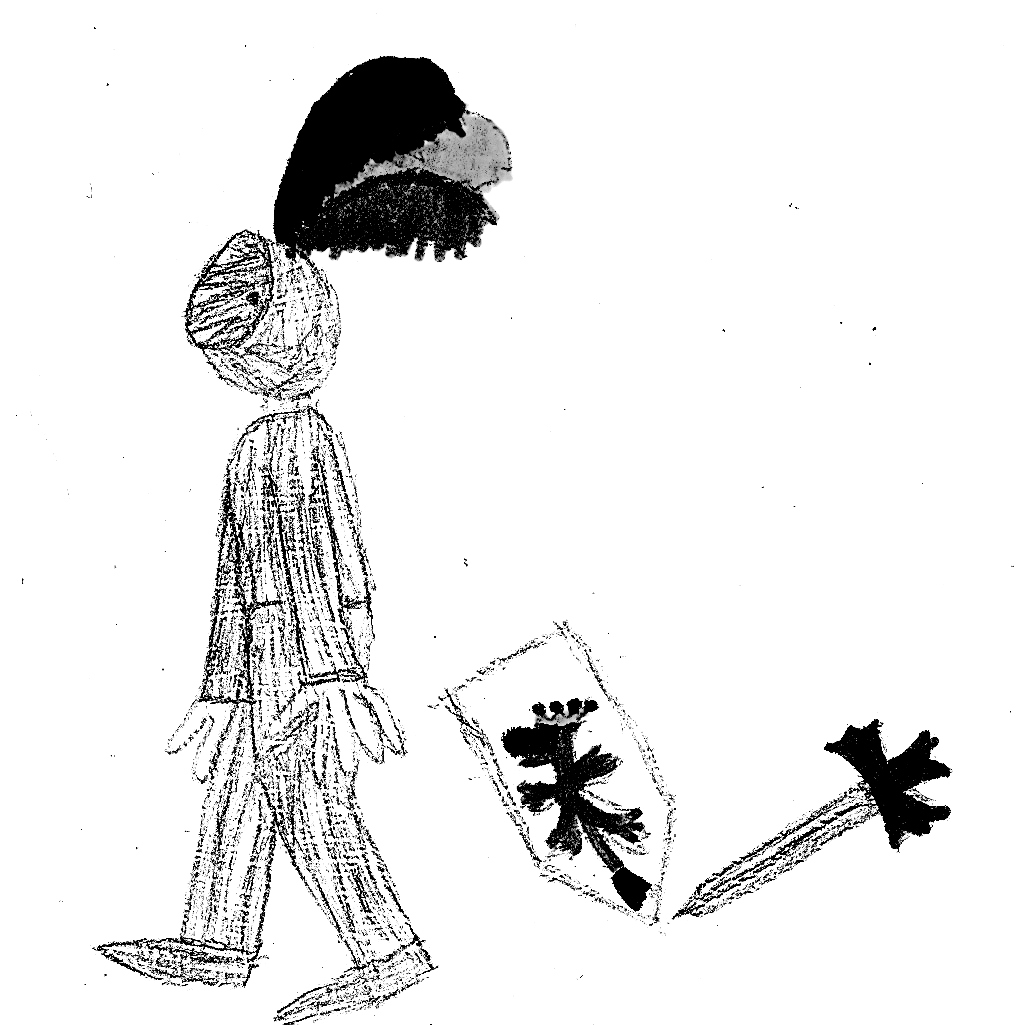
\includegraphics[width=6cm]{pict/asi-rytíř.jpg}
\end{center}
\end{song}

\pagebreak
\begin{song}{Omnia vincit amor}{F}{Klíč}

\begin{SBVerse}

\Ch{dmi}{Šel} pocestný kol \Ch{C}{hospodských} \Ch{dmi}{zdí,}

\Ch{F}{přisedl} k nám a \Ch{C}{lokálem} \Ch{F}{zní}

\Ch{gmi}{pozdrav} jak svaté \Ch{F}{při}kázá\Ch{C}{ní:}

\Ch{dmi}{Omnia} \Ch{C}{vincit} \Ch{dmi}{Amor.}

\end{SBVerse}

\begin{SBVerse}

Hej, šenkýři, dej plný džbán,

ať chasa ví, kdo k stolu je zván,

se mnou ať zpívá, kdo za své vzal

Omnia vincit Amor.

\end{SBVerse}

\begin{SBChorus}

Zlaťák \Ch{F}{pálí,} \Ch{C}{nesleví} \Ch{dmi}{nic,}

štěstí v \Ch{F}{lásce} \Ch{C}{znamená} \Ch{F}{víc,}

všechny \Ch{gmi}{pány} \Ch{F}{ať }vezme \Ch{C}{ďas!} \Ch{A7}{}

\Ch{dmi}{Omnia} \Ch{C}{vincit} \Ch{dmi}{Amor.}

\end{SBChorus}

\begin{SBVerse}

Já viděl zemi válkou se chvět,

musel se bít a nenávidět,

v plamenech pálit prosby a pláč -

Omnia vincit Amor.

\end{SBVerse}

\begin{SBVerse}

Zlý trubky troubí, vítězí zášť,

nad lidskou láskou roztáhli plášť,

vtom kdosi krví napsal ten vzkaz:

Omnia vincit Amor.

\end{SBVerse}
\begin{SBChorus}

\end{SBChorus}
\begin{SBVerse}

Já prošel každou z nejdelších cest,

všude se ptal, co značí ta zvěst,

až řekl moudrý: "Pochopíš sám,

všechno přemáhá láska."

\end{SBVerse}

\begin{SBVerse}

Teď s novou vírou obcházím svět,

má hlava zšedla pod tíhou let,

každého zdravím tou větou všech vět:

Omnia vincit Amor.\end{SBVerse}

\end{song}

\pagebreak
\begin{song}{Pánové nahoře}{C}{Jaromír Nohavica}

\begin{SBVerse}

1. \Ch{C}{Pánové} naho\Ch{emi}{ře,} já \Ch{dmi7}{píšu} vám dnes \Ch{G7}{psaní}

a \Ch{dmi7}{nevím} vlastně \Ch{C}{ani,} bu\Ch{dmi7}{dete-li} ho \Ch{G7}{číst,}

\Ch{C}{přišlo} mi ve \Ch{emi}{středu} do \Ch{dmi7}{války} předvo\Ch{G7}{lání,}

je \Ch{dmi7}{to bez} odvo\Ch{C}{lání, }tím \Ch{dmi7}{prý} si \Ch{G7}{mám} být \Ch{C}{jist.}

\Ch{F}{Pánové} nahoře, \Ch{Cdim}{já už }to lejstro \Ch{emi}{spálil,}

už \Ch{Ami}{jsem} si kufry \Ch{dmi7}{sbalil,} správcové vrátil \Ch{G7}{klíč,}

\Ch{C}{pánové} \Ch{emi}{nahoře,} uc\Ch{dmi7}{tivě} se vám \Ch{G7}{klaním}

a \Ch{dmi7}{zítra} vlakem \Ch{C}{ranním} \Ch{dmi7}{odjíždím} \Ch{G7}{někam} \Ch{C}{pry}\Ch{emi}{č.} \Ch{dmi7}{} \Ch{G7}{}
\end{SBVerse}

\begin{SBVerse}
Co už jsem na světě, viděl jsem zoufat matky

nad syny, kteří zpátky se nikdy nevrátí,

slyšel jsem dětský pláč a viděl jejich slzy,

které snadno a brzy se z očí neztratí.

Znám vaše věznice, znám vaše kriminály,

i ty, kterým jste vzali život či minulost,

vím také, že máte solidní arzenály,

i když jste povídali o míru víc než dost.
\end{SBVerse}

\begin{SBVerse}
Pánové nahoře, říká se, že jste velcí

a na věci to přece vůbec nic nemění,

pánové nahoře, na to jste vážně malí,

abyste vydávali rozkazy k vraždění.

Musí-li války být, běžte si válčit sami

a vaši věrní s vámi, mě, mě nechte být,

jestli mě najdete, můžete klidní být,

střílejte, neváhejte, já zbraň nebudu mít\dots
\end{SBVerse}

\end{song}

\pagebreak
\setcounter{page}{66}
\begin{song}{Pískající cikán}{G}{Spiritual kvintet}

\begin{SBVerse}

\Ch{G}{Dívka} \Ch{ami}{loudá} se \Ch{G}{vinicí}\Ch{ami}{,}\Ch{G}{tam,} kde \Ch{ami}{zídka} je \Ch{hmi}{nízk}\Ch{ami}{á,}

\Ch{G}{tam,} kde \Ch{ami}{stráň} končí \Ch{hmi}{vonící,}\Ch{C}{tam} \Ch{G}{písnič}\Ch{C}{ku} někdo \Ch{G}{pí}\Ch{C}{sk}\Ch{D}{á.}

\end{SBVerse}

\begin{SBVerse}

Ohlédne se a "Propána!", v stínu, kde stojí líska,

švárného vidí cikána, jak leží, písničku píská.

\end{SBVerse}

\begin{SBVerse}

Chvíli tam stojí potichu, písnička si jí získá,

domů jdou spolu do smíchu, je slyšet cikán, jak píská.

\end{SBVerse}

\begin{SBVerse}

Jenže tatík, jak vidí cikána, pěstí do stolu tříská,

"Ať táhne pryč, vesta odraná, groš nemá, něco ti spíská."

\end{SBVerse}

\begin{SBVerse}

Teď smutnou dceru má u vrátek, jen Bůh ví, jak se jí stýská,

"kéž vrátí se mi zas nazpátek ten který v dálce si píská."

\end{SBVerse}

\begin{SBVerse}

Pár šidel honí se po louce, v trávě rosa se blýská,

cikán, rozmarýn v klobouce, jde dál a písničku píská.

\end{SBVerse}

\begin{SBVerse}

Na závěr zbývá už jenom říct, v čem je ten kousek štístka:

peníze často nejsou nic, má víc, kdo po svém si píská ...

\end{SBVerse}

\end{song}

\pagebreak

\setcounter{page}{68}
\begin{song}{Pošťák}{C}{Hop Trop}
\begin{SBVerse}
\Ch{ami}{Psal jsem ti, }\Ch{G}{brácho, a }\Ch{ami}{na ouřad }\Ch{G}{psaní šel }\Ch{F}{dát,}

psaní vo \Ch{C}{tom,} že jsem \Ch{dmi}{černej}, že z \Ch{ami}{fleku} bych \Ch{E7}{krad',}

z \Ch{ami}{váčku jsem }\Ch{G}{lovil pár }\Ch{ami}{centů a }\Ch{G}{šéf mi vtom }\Ch{F}{řek':}

pošťák se \Ch{C}{nevrátil, }\Ch{dmi}{jestli bych }\Ch{ami}{vzal po něm }\Ch{E7}{flek,}

\Ch{ami}{sáně mi }\Ch{G}{dal, tresky v }\Ch{ami}{balíku }\Ch{G}{pro psy a }\Ch{F}{kvér,}

brašnu, v ní \Ch{C}{lejstra, a }\Ch{dmi}{po zádech }\Ch{ami}{plác}' mi: Buď \Ch{E7}{fér!}
\end{SBVerse}
\begin{SBChorus}
\Ch{A}{Pošťák se má, za }\Ch{D}{známky nepla}\Ch{A}{tí,}

\Ch{D}{hlavně když se s }\Ch{C}{pytlem prachů }\Ch{E7}{někam neztra}\Ch{A}{tí,}

pošťák se má, a \Ch{D}{když se neztra}\Ch{A}{tí,}

\Ch{D}{za pět roků }\Ch{C}{utopený }\Ch{E7}{sáně zapla}\Ch{A}{tí.}
  \end{SBChorus}
\begin{SBVerse}
Ten rok byl divnej, i slunce si přišlo ňák dřív,

led se měl hnout, a když ne, tak to stal by se div,

místo jsem našel, kde předjíždět Kobuk měl jít,

dál předák nechtěl a já nerad musel psy bít,

zázrakem živej pak dostal se na druhej břeh

bez psů a sání, a proklínal zbytečnej spěch.
\end{SBVerse}
\end{song}

\pagebreak

\begin{song}{Prasátko}{G}{Buty}

\Ch{$|$:}{} \Ch{G}{} \Ch{C}{} \Ch{B}{} \Ch{D}{} \Ch{:$|$}{}
\begin{SBVerse}
\Ch{G}{Přišlo za mnou }\Ch{C}{jedno malé }\Ch{B}{prasátko}\Ch{D}{,}

\Ch{G}{že už se mu }\Ch{C}{nelíbí být }\Ch{B}{prasátko}\Ch{D}{}

\Ch{Emi}{Mazlil jsem se s }\Ch{G}{ním, s }\Ch{C}{tím prasátkem }\Ch{D}{maličkým}

\Ch{G}{chrochtalo mi }\Ch{Ami}{něco }\Ch{D7}{do }\Ch{G}{uší}\Ch{C}{ }\Ch{D}{}

\end{SBVerse}

\begin{SBVerse}

Měl jsem uši oslintané prasátkem,

které potom zase rychle uteklo.

Někam za láskou a já se trápím otázkou,

co chtělo to malé prasátko.

Někam za láskou a já se trápím otázkou,

co chtělo to malé prasátko.

\end{SBVerse}

\end{song}

\pagebreak
\begin{song}{Rána v trávě}{C}{Žalman}

(Capo 3)
\begin{SBChorus}
\Ch{ami}{Každý ráno boty }\Ch{G}{zouval }\Ch{ami}{Orosil si nohy v }\Ch{G}{trávě}

\Ch{ami}{Že se lidi mají radi }\Ch{G}{doufal }\Ch{ami}{A pro}\Ch{emi}{citli }\Ch{ami}{právě}

\Ch{ami}{Každý ráno dlouze }\Ch{G}{zíval }\Ch{ami}{Utřel čelo do ru}\Ch{G}{kávu}

\Ch{ami}{A při chůzi tělem semtam }\Ch{G}{kýval }\Ch{ami}{Před se}\Ch{emi}{bou sta }\Ch{ami}{sáhů}
\end{SBChorus}
\begin{SBVerse}
\Ch{C}{Poznal }\Ch{G}{Mora}\Ch{F}{věnku }\Ch{C}{krásnou}

\Ch{ami}{a ví}\Ch{G}{nečko }\Ch{C}{ze zlata}

\Ch{C}{V Čechách }\Ch{G}{slávu }\Ch{F}{muzi}\Ch{C}{kantů}

\Ch{ami}{Uma}\Ch{emi}{zanou }\Ch{ami}{od bláta.}
\end{SBVerse}
\begin{SBVerse}
Toužil najít studánečku

A do ní se podívat

By mu řekla proč holečku

Musíš světem chodívat
\end{SBVerse}
\begin{SBVerse}
Studánečka promluvila

To ses musel nachodit

Abych já ti pravdu řekla

měl ses jindy narodit.
\end{SBVerse}
\end{song}

\pagebreak
\begin{song}{Ryl jen, celej den ryl}{C}{Spiritual kvintet}
\begin{SBVerse}
Já \Ch{ami}{každý ráno v sedm hodin vstal}

a \Ch{E7}{krumpáč s lo}\Ch{ami}{pato}\Ch{E7}{u vyfasoval,}

pak s pa\Ch{ami}{rtou, která makat dovede,}

jsem do\Ch{E}{šel tam, co tunel povede.}
\end{SBVerse}
\begin{SBChorus}
\Ch{E7}{A} \Ch{ami}{ryl jen, ce}\Ch{E7}{lej den }\Ch{ami}{ryl,} já ryl jen, ce\Ch{G}{lej den }\Ch{ami}{ryl,}

abych dřív, než do svý \Ch{C}{boudy pudu }\Ch{E7}{spát,}

\Ch{ami}{čaj v kantý}\Ch{Ami/G}{ně} \Ch{Ami/F}{moh' si} \Ch{E7}{dát,}

já \Ch{ami}{ryl jen, ce}\Ch{E7}{lej den }\Ch{ami}{ryl, celej den,}

\Ch{E7}{jak kr}\Ch{ami}{tek celej den }\Ch{E7}{jen ry}\Ch{ami}{l.}

\Ch{$|$:}{} \Ch{A}{} \Ch{G}{} \Ch{F}{} \Ch{E}{} \Ch{:$|$}{}

\end{SBChorus}
\begin{SBVerse}
Kdo netrhal skálu, těžko pochopí,

co sám dynamit někdy natropí,

když jednou náhle došlo k výbuchu,

Jim Goff vyletěl majli do vzduchu.
\end{SBVerse}
\begin{SBVerse}
A když z tý vejšky zas na zem si kec',

předák McCane ho popad' za límec:

"Tak se mi zdá, že línej jsi jak veš,

mně ve vzduchu se flákat nebudeš!"
\end{SBVerse}
\begin{SBVerse}
Teď po létech, když večer sedím sám,

na starý dobrý časy vzpomínám,

zas slyším tmou, jak rány duněly,

když ve skalách jsem lámal tunely.
\end{SBVerse}
\end{song}

\pagebreak
\begin{song}{Sáro}{C}{Traband}

\begin{SBVerse}

Sbor \Ch{ami}{kajícných} \Ch{emi}{mnichů} \Ch{F}{jde} krajinou \Ch{C}{v }tichu 

a pro \Ch{F}{vše}chnu lidskou \Ch{C}{pýc}hu má jen \Ch{F}{přezíravý} \Ch{G}{smích.}

A z prohraných válek se vojska domů vrací 

však zbraně stále burácí a bitva zuří v nich.

\end{SBVerse}

\begin{SBChorus}

Sáro, Sáro, v noci se mi zdálo, 

že tři andělé boží k nám přišli na oběd. 

Sáro, Sáro, jak moc anebo málo 

mi chybí abych tvijí duši mohl rozumět.

\end{SBChorus}

\begin{SBVerse}

Vévoda v zámku čeká na balkóně 

až přivedou mu koně, pak mává na pozdrav. 

Srdcová dáma má v každé ruce růže, 

tak snadno pohřbít může sto urozených hlav.

\end{SBVerse}

\begin{SBVerse}

Královnin šašek s pusou od povidel 

sbírá zbytky jídel a myslí na útěk. 

A v podzemí skrytí slepí alchymisté 

už oběvili jistě proti povinnosti lék!

\end{SBVerse}

\begin{SBVerse}

Páv pod tvým oknem zpívá sotva procit 

o tajemstvích noci ve tvých zahradách. 

A já, potulný kejklíř, co svázali mu ruce, 

teď hraju o tvé srdce a chci mít tě nadosah!

\end{SBVerse}

\begin{SBChorus}

Sáro, Sáro, pomalu a líně 

s hlavou na tvém klíně chci se probouzet. 

Sáro, Sáro, Sáro, Sáro rosa padá ráno 

a v poledne už možná bude jiný svět!

\end{SBChorus}

\begin{SBVerse}

Sáro, Sáro, vstávej milá Sáro, 

\Ch{F}{andělé} k nám \Ch{dmi}{přišli} na \Ch{Cmaj}{oběd.}

\end{SBVerse}

\end{song}

\pagebreak
\setcounter{page}{78}
\begin{song}{Severní vítr}{C}{Zdeněk Svěrák a Jaroslav Uhlíř}

\begin{SBVerse}

Jdu s \Ch{C}{děravou patou, mám }\Ch{ami}{horečku} zlatou

Jsem \Ch{F}{chudý, jsem sláb a }\Ch{C}{nemocen}

Hlava mě pálí a v \Ch{ami}{modravé dáli}

Se \Ch{F}{leskne a }\Ch{G7}{třpytí můj }\Ch{C}{sen}

\end{SBVerse}

\begin{SBVerse}

Kraj pod sněhem mlčí, tam stopy jsou vlčí

Tam zbytečně budeš mi psát

Sám v dřevěné boudě sen o zlaté hroudě

Já nechám si tisíc krát zdát

\end{SBVerse}

\begin{SBChorus}

\Ch{C}{Severní }\Ch{C7}{vítr je }\Ch{F}{krutý,} \Ch{C}{ počítejlásko má s }\Ch{G7}{tím}

\Ch{C}{k nohám ti }\Ch{C7}{dám zlaté }\Ch{F}{pruty} nebo se \Ch{C}{vůbec }\Ch{G7}{nevrá}\Ch{C}{tím}

\end{SBChorus}

\begin{SBVerse}

Tak zarůstám vousem a vlci už jdou sem

Už slyším je výt blíž a blíž

už mají mou stopu, už větří že kopu

svůj hrob a že stloukám si kříž

\end{SBVerse}

\begin{SBVerse}

Zde leží ten blázen, chtěl dům a chtěl bazén

A opustil tvou krásnou tvář

Má plechovej hrnek a pár zlatejch zrnek

Nad hrobem polární zář.

\end{SBVerse}

\end{song}

\pagebreak

\begin{song}{Sirka}{G}{Demophobia}

\Ch{[ Emi}{} \Ch{C}{} \Ch{D}{} \Ch{G]}{}

\begin{SBChorus*}

Našel jsem doma starou sirku

ta sirka byla vypálená

zavolal jsem si bratra Jirku:

„Jirko ta sirka byla má!“

\end{SBChorus*}

\begin{SBChorus*}
\begin{itshape}
On řekl: „Ty mě houpáš!“

Já na to: „Tak jest!“

On řekl: „Tak mě přesvědč!“

Já na to: „Pojď ven!“
\end{itshape}
\end{SBChorus*}

\begin{SBChorus*}

A tak jsme šli do garáže

táta tam má žiguli

koupil ho ze svý apanáže

můj táta je lidumil

\end{SBChorus*}

\begin{SBChorus*}
\begin{itshape}
On řekl: „Proč jsme tady!“

Já na to: „Ty nekecej!“

On řekl: „Já nic, já nic!“

Já na to: „Pojď sem!“
\end{itshape}
\end{SBChorus*}

\begin{SBChorus*}

Svázal jsem ho do kozelce

pak ho polil benzínem

chvíli dělal kotrmelce

to než se stal plamenem

\end{SBChorus*}

\begin{SBChorus*}
\begin{itshape}
On řekl: „Ty jsi blázen!“

Já na to: „Cože?“

On řekl: “Ahoj brácho!“

Já na to: „Sbohem!“
\end{itshape}
\end{SBChorus*}

\begin{SBChorus*}

Našel jsem doma starou sirku

ta sirka byla vypálená

už nemám, nemám bratra Jirku

za to může sirka má…

\end{SBChorus*}

\end{song}

\pagebreak
\input{song/a_slavíci-z-madridu.tex}
\setcounter{page}{83}
\begin{song}{Stýskání}{D}{Bratři Ebenové}
\begin{SBVerse}
\Ch{A}{Stýská} se \Ch{D}{mi}, \Ch{emi}{černovlás}\Ch{hmi}{ko}, \Ch{f#mi}{po} louče\Ch{hmi}{ní}, \Ch{G}{kdy} jsi se \Ch{A}{mi} 

\Ch{f#mi}{na} rame\Ch{hmi}{ni} \Ch{G}{vyplaka}\Ch{C}{la,} černovlás\Ch{A}{ko.}\Ch{emi7}{}\Ch{A}{}

\end{SBVerse}
\begin{SBVerse}

Stýská se mi, černovlásko, po toužení, kdy jsi se mi

něžně smála, rozespalá, černovlásko.

\end{SBVerse}
\begin{SBChorus}
\Ch{hmi}{Stýská} -- \Ch{G}{šest} písmen \Ch{D}{místo} Tvé \Ch{A}{lásky},

\Ch{emi}{stýská} -- \Ch{f#mi}{pláčou} dlou\Ch{hmi}{hé} samo\Ch{f#mi}{hlásky,}

\Ch{hmi}{stýská} -- \Ch{G}{zůstala} \Ch{D}{jsi} mi pod \Ch{A}{víčky,}

\Ch{hmi}{dohořel} knot svíčky, \Ch{Gmaj7}{uschly} tvé slzičky

\Ch{emi7}{a }dveří skřípání nese mi \Ch{A}{stýskání}.

  \end{SBChorus}
\begin{SBVerse}
Stýská se mi, černovlásko, rád jsem stonal ve tvém klíně,

podleh' tobě i angíně, černovlásko.
\end{SBVerse}
\begin{SBVerse}

Stýská se mi, černovlásko, po snídání v deset ráno,

proč máme dnes vyprodáno, černovlásko?

  \end{SBVerse}
  \begin{SBVerse}
Stýská se mi, černovlásko, po tvé rtěnce perleťové,

na ústa mě už neklove, černovlásko.

\end{SBVerse}
\begin{SBVerse}

Stýská se mi, černovlásko, smutný je čas účtování,

inventura milování, černovlásko.

  \end{SBVerse}
\begin{SBChorus*}
 $|$: \Ch{A}{Stýská} se \Ch{D}{mi}, \Ch{emi}{hm}, \Ch{hmi}{} \Ch{f#mi}{stýská} se \Ch{hmi}{mi}, \Ch{G}{hm,}
 \Ch{Asus4}{ \dots :$|$} 
 \end{SBChorus*}
 \end{song}

\pagebreak

\setcounter{page}{85}
\begin{song}{Tereza}{G}{Wabi Ryvola}

\begin{SBVerse}

\Ch{G}{Ten }\Ch{C}{den co vítr }\Ch{D}{listí z města }\Ch{G}{svál}

můj \Ch{C}{džíp se vracel }\Ch{D}{jako by se }\Ch{emi}{bál}

že \Ch{C}{asfaltový }\Ch{D}{moře odliv }\Ch{G}{má}

a \Ch{C}{stáj, že svýho }\Ch{D}{koně }\Ch{E7}{nepozná.}

\end{SBVerse}

\begin{SBChorus}

\Ch{G}{Řekni kolik je na světě kolik je takovejch }\Ch{D}{měst}

řekni \Ch{ami}{kdo by se vracel když všude je tisíce }\Ch{emi}{cest.}

Tenkrát \Ch{G}{když jsi mi Terezo řekla že ráda mě }\Ch{D}{máš}

tenkrát \Ch{ami}{ptal jsem se Terezo kolik mi polibků }\Ch{emi}{dáš,}

napos\Ch{D}{led, napos}\Ch{G}{led.}

\end{SBChorus}

\begin{SBVerse}

Já z dálky viděl město v slunci stát

a dál jsem se jen s hrůzou mohl ptát.

Proč vítr mlátí spoustou okenic?

Proč jsou v ulici auta, jinak nic?

\end{SBVerse}

\begin{SBVerse}

Do prázdnejch beden zotvíranejch aut

zaznívá odněkud něžný tón Flaut

a v závěji starýho papíru

válej se černý klapky z klavírů.

\end{SBVerse}

\begin{SBVerse}

Tak loudám se tím hrozným městem sám

a vím že Terezu už nepotkám.

Jen já tu zůstal s prázdnou ulicí

a vosamělý město mlčící.

\end{SBVerse}

\end{song}

\pagebreak

\begin{song}{Topič}{C}{Karel Plíhal}

\begin{SBVerse}

Sedí \Ch{C}{topič u piána, prelud}\Ch{emi}{uje potají}

a pod p\Ch{G}{rsty toho pána bílé kl}\Ch{C}{apky č}\Ch{D9/F#}{ernají}\Ch{G}{.}

Za ta \Ch{C}{léta u divadla, která str}\Ch{emi}{ávil v kotelně,}

hraje sv\Ch{G}{oje "Pec nám spadla" stále v}\Ch{C}{íce f}\Ch{F7}{orteln}\Ch{C}{ě.}

\end{SBVerse}

\begin{SBChorus}

\Ch{cmi4}{Zatímco se hudebníci v}\Ch{F}{ybavují u kávy,}

t\Ch{D7}{opič si nad klávesnicí v}\Ch{G}{yhrnuje r}\Ch{G#}{ukáv}\Ch{G}{y.}

\end{SBChorus}

\begin{SBVerse}

Sedí topič u piána, preluduje potají

a pod prsty toho pána bílé klapky černají.

Slaví celý rozesmátý konec topné sezóny

a kysličník uhelnatý proměnil se na tóny.

\end{SBVerse}

\end{song}

\pagebreak
\setcounter{page}{89}
\begin{song}{Topoly}{C}{Ondřej Balík}
\begin{SBChorus*}
\Ch{hmi}{Jako} ty topoly máme svý stíny, žijeme ze soli vody a hlíny.
\end{SBChorus*}
\begin{SBVerse}
\Ch{ami}{Jako} ty topoly \Ch{dmi7}{stojíme} vzpříma, 

\Ch{Cmaj}{dokud} nám dovolí s\Ch{F}{lunce} a z\Ch{F}{im}\Ch{E}{a},

\Ch{ami}{jako} ty topoly \Ch{dmi7}{celí se} třesem,

\Ch{Cmaj}{sekyra} zabolí, s\Ch{hmi7}{ekyra} zabolí,

\Ch{F}{znamení} \Ch{F}{ne}\Ch{E}{sem}.

\Ch{ami}{Jako} ty topoly, \Ch{dmi7}{když} nemáš sílu,

\Ch{Cmaj}{tak} lidi z okolí \Ch{F}{přinesou} \Ch{F}{pil}\Ch{E}{u}.

\Ch{ami}{Jako} ty topoly \Ch{dmi7}{v} pláči a křiku,

\Ch{Cmaj}{bouře} tě oholí, \Ch{hmi7}{bouře} tě oholí

\Ch{G4}{do} vykřiční\Ch{F#4}{ku}.
\end{SBVerse}
\begin{multicols}{2}
\begin{scriptsize}
\begin{SBVerse}
Jako ty topoly strach někde nízko,

v nejhlubším údolí k nebi máš blízko.

Jako ty topoly horko nás moří,

belháš se o holi, belháš se o holi,

za tebou hoří.

Jako ty topoly až přejde září,

strniště na poli, listí a stáří.

Jako ty topoly do příští zimy,

koho to zabolí, koho to zabolí,

budou tu jiní.
%sloka 2
\end{SBVerse}
[:h03e232h3e012:][hmi G A f\#mi]
\begin{SBVerse}
Jako ty topoly, jako ty stromy,

jeden si dovolí, jinej se zlomí.

Jako ty topoly máme svý stíny,

žijeme ze soli, vody a hlíny.

Jako ty topoly, jako ty stromy,

jeden si dovolí, jinej se zlomí.

Jako ty topoly máme svý stíny,

žijeme ze soli, vody a hlíny.

Jako ty topoly, jako ty stromy,

jeden si dovolí, jinej se zlomí.

Jako ty topoly máme svý stíny,

žijeme ze soli, vody a hlíny.

Jako ty ...
%sloka 3
\end{SBVerse}
\end{scriptsize}
\end{multicols}
\end{song}

\pagebreak

\begin{song}{Trampská}{F}{Bratři Ebenové}

\begin{SBVerse}

\Ch{dmi}{Mlhavým ránem bose jdou, kanady vržou na nohou}

a dálka tolik vzdále\Ch{G}{ná je }\Ch{dmi}{blízká,}

město jsi nechal za zády, zajíci dělaj' rošády

a v křoví někdo tiše \Ch{G}{Vlajku }\Ch{dmi}{píská,}

\Ch{G}{najednou} připadáš si ňák príma, svobodnej, a tak,

tak \Ch{dmi}{ňák, tak }\Ch{G}{ňák, ňák }\Ch{dmi}{tak.}

\end{SBVerse}

\begin{SBChorus}

Pojď \Ch{F}{dál,} s námo se nenudíš, pojď dál, ráno se probudíš,

a vedle sebe máš o šišku \Ch{dmi}{víc,}

pojď \Ch{F}{dál,} pod sebou pevnou zem, pojď dál, a Číro 

s Melounem a Meky, Miky, Vrt, a dál už \Ch{G}{nic, dál už }\Ch{dmi}{nic.}

\end{SBChorus}

\begin{SBVerse}

Mlhavý ráno za tratí, u cesty roste kapratí,

sbalíš si deku, spacák, celtu, pytel,

a kdyby ňákej úředník začal ti říkat, co a jak,

sbalíš si deku, spacák, celtu, pytel,

důležitý je to, co jseš, odkud jsi přišel a kam jdeš,

co jseš, kam jdeš, co jseš.

\end{SBVerse}

\end{song}

\pagebreak
\begin{song}{Tři kříže}{C}{Hop trop}

\begin{SBVerse}

\Ch{dmi}{Dávám sbohem }\Ch{C}{břehům prokla}\Ch{ami}{tejm,}

který \Ch{dmi}{v drápech má }\Ch{C}{ďábel }\Ch{dmi}{sám.}

\Ch{dmi}{Bílou přídí }\Ch{C}{šalupa „My }\Ch{ami}{grave“}

míří \Ch{dmi}{k útesům, }\Ch{C}{který }\Ch{dmi}{znám.}

\end{SBVerse}

\begin{SBChorus}

Jen tři \Ch{F}{kříže z bí}\Ch{C}{lýho kame}\Ch{ami}{ní}

někdo \Ch{dmi}{do písku }\Ch{C}{posklá}\Ch{dmi}{dal.}

Slzy \Ch{F}{v očích měl a }\Ch{C}{v ruce znave}\Ch{ami}{ný,}

lodní \Ch{dmi}{deník, co }\Ch{C}{sám do něj }\Ch{dmi}{psal.}

\end{SBChorus}

\begin{SBVerse}

První kříž má pod sebou jen hřích, 

samý pití a rvačka jen.

Chřestot nožů. při kterých přejde smích, 

srdce kámen a jméno „Sten“.

\end{SBVerse}

\begin{SBVerse}

Já Bob Green, mám tváře zjizvený, 

štěkot psa zněl, když jsem se smál,

Druhej kříž mám a spím pod zemí, 

že jsem falešný karty hrál.

\end{SBVerse}

\begin{SBVerse}

Třetí kříž sand vyvolá jen vztek, 

Katty Rodgers těm dvoum život vzal.

Svědomí měl vedle nich si klek ...

\end{SBVerse}

Rec: Vím, trestat je lidský, ale odpouštět božský. 

Ať mi tedy Bůh odpustí.
\end{song}

\pagebreak
\setcounter{page}{94}
\begin{song}{Tulácký ráno}{F}{Jan Nedvěd}

\begin{SBVerse}

\Ch{dmi}{Posvátný je mi každý ráno,}

\Ch{ami}{když} ze sna budí \Ch{ami7}{šumící }\Ch{dmi}{les}

a když se zvedám s písničkou známou

a přezky chřestí o skalnatou mez.

\end{SBVerse}

\begin{SBChorus}

\Ch{dmi}{Tulácký} ráno, na kemp se snáší,

\Ch{B}{za chvíli půjdem }\Ch{C}{toulat se }\Ch{F}{dál,}

\Ch{dmi}{a vodou z říčky oheň se zháší,}

\Ch{B}{tak zase půjdem }\Ch{C}{toulat se }\Ch{dmi}{dál.}\Ch{Dsus2}{}

\end{SBChorus}

\begin{SBVerse}

Posvátný je mi každý večer

když oči k ohni vždy vrací se zpět

Tam mnohí z pánů měl by se kouknout

a hned by viděl, jakej chcem svět.

\end{SBVerse}

\begin{SBVerse}

Posvátný je mi každý slovo,

když lesní moudrost a přírodu znáš,

bobříku sílu a odvahu touhy

kolik v tom pravdy, však kdo nám ji dá ?

\end{SBVerse}

\end{song}

\pagebreak

\setcounter{page}{95}
\begin{song}{Už to nenapravím}{C}{Jaroslav Samson Lenk}

\begin{SBChorus}

\Ch{ami}{Vap }\Ch{D}{tada} \Ch{F}{dap} \Ch{E7}{\dots} \Ch{ami}

\end{SBChorus}

\begin{SBVerse}

V \Ch{ami}{devět hodin dvacet pět }\Ch{D}{mě opustilo štěstí,}

ten \Ch{F}{vlak, co jsem jím měl jet, na koleji }\Ch{E}{dávno }\Ch{E7}{nestál,}

v devět hodin dvacet pět jako bych dostal pěstí,

já za hodinu na náměstí měl jsem stát,

ale v jiným městě.

Tvá \Ch{A}{zpráva} zněla prostě a \Ch{A7}{byla tak krátká,}

že \Ch{fmi}{stavíš se jen na skok, že nechalas' mi vrátka}

\Ch{G}{zadní otevřená, }\Ch{E}{zadní otevřená,}

já naposled tě viděl, když ti bylo dvacet,

to jsi tenkrát řekla, že se nechceš vracet,

že jsi unavená, ze mě unavená.

\end{SBVerse}

\begin{SBVerse}

Já čekala jsem, hlavu jako střep, a zdálo se, že dlouho,

snad může za to vinný sklep, že člověk často sleví,

já čekala jsem, hlavu jako střep, s podvědomou touhou,

já čekala jsem dobu dlouhou, víc než dost, 

kolik přesně, nevím.

Pak jedenáctá byla a už to bylo passé,

já dřív jsem měla vědět, že vidět tě chci zase,

láska nerezaví, láska nerezaví.

Ten dopis, co jsem ti psala, byl dozajista hloupý,

byl odměřený moc na vlídný slovo skoupý,

už to nenapravím, už to nenapravím.

\end{SBVerse}
\end{song}

\pagebreak

\begin{song}{Válka Růží}{F}{Spiritual Kvintet}
\begin{SBVerse}
Už \Ch{dmi}{rozplynul se }\Ch{G}{hustý dým,} \Ch{dmi}{derry down, hej, }\Ch{A}{down-a-down,}

nad zti\Ch{dmi}{chlým polem vá}\Ch{gmi}{lečným, derry do}\Ch{dmi}{wn,} \Ch{A}{}

jen \Ch{F}{ticho stojí }\Ch{C}{kolko}\Ch{A}{lem}

a ví\Ch{dmi}{těz ple}\Ch{dmi/C}{ní vla}\Ch{B}{stní }\Ch{A}{zem,}

je válka rů\Ch{dmi}{ží, down,} \Ch{gmi}{derry, derry, }\Ch{A}{derry down-a-}\Ch{dmi}{down.}
\end{SBVerse}
\begin{SBVerse}
Nečekej soucit od rváče, derry down, hej, down-a-down,

kdo zabíjí ten nepláče, derry down,

na těle mrtvé krajiny,

se mečem píšou dějiny,

je válka růží, down, derry, derry, derry down, a-down.
\end{SBVerse}
\begin{SBVerse}
Dva erby, dvojí korouhev, derry down, hej, down-a-down,

dva rody živí jeden hněv, derry down,

kdo změří, kam se nahnul trůn, 

zda k Yorkům nebo k Lancastrům,

je válka růží, down, derry, derry, derry down, a-down.
\end{SBVerse}
\begin{SBVerse}
Dva erby, dvojí korouhev, derry down, hej, down-a-down,

však hlína pije jednu krev, derry down,

ať ten či druhý přežije, 

vždy nejvíc ztratí Anglie,

je válka růží, down, derry, derry, derry down, a-down.
\end{SBVerse}
\end{song}

\pagebreak
\begin{song}{Velrybářská výprava}{C}{Antonín Linhart}

\begin{SBVerse}

\Ch{C}{Jednou plác mě přes }\Ch{F}{rameno Joh}\Ch{G}{ny zvanej \Ch{C}{Knecht}:}

\Ch{ami}{Mám pro tebe, ho}\Ch{dmi}{chu, v pácu moc }\Ch{G}{fajnovej }\Ch{C}{kšeft!}

\Ch{C}{Objednal} hned litr \Ch{F}{rumu a }\Ch{G}{pak nežně }\Ch{C}{řval:}

\Ch{ami}{Sbal se, jedem na }\Ch{dmi}{velryby, prej }\Ch{G}{až za po}\Ch{C}{lár.}

\end{SBVerse}

\begin{SBChorus}

$|$: Výprava vel\Ch{C}{rybářská kole}\Ch{F}{m Grónska nez}\Ch{G}{dařila se,}

\Ch{C}{protože} nejeli \Ch{ami}{jsme na vel}\Ch{dmi}{ryby, ale }\Ch{G}{na mro}\Ch{C}{že.} :$|$

\end{SBChorus}

\begin{SBVerse}

Briga zvaná Malá Kitty kotví v zátoce,

nakládaj se sudy s rumem, maso, ovoce,

vypluli jsme časne zrána, smer severní pól,

dřív, než přístav zmizel z očí, každej byl namol.

\end{SBVerse}

\begin{SBVerse}

Na loď padla jinovatka, s ní třeskutej mráz,

hoň velryby v kupách ledu, to ti zlomí vaz,

na pobreží místo ženskejch mávaj tučňáci,

v tomhle kraji beztak nemáš jinou legraci.

\end{SBVerse}

\begin{SBVerse}

Když jsme domú připluli, už psal se přítí rok,

starej řejdař povídá, že nedá ani flok:

Místo velryb v Grónským moři zajímal vás grog,

tuhle práci zaplatil by asi jenom cvok.

\end{SBVerse}

\begin{SBVerse}

Tohleto nám neměl říkat, teď to dobře ví,

stáhli jsme mu kuži z těla, tomu hadovi,

z paluby pak slanej vítr jeho tělo smet, chachacha,

máme velryb plný zuby, na to vezmi jed.

\end{SBVerse}

\end{song}

\pagebreak
\begin{song}{Vlajka}{F,D}{Jan Korda}
\begin{SBVerse}
Vše tone v \Ch{dmi}{snách} a život kolem \Ch{A}{ztich, }

jen dole v \Ch{A7}{tmách} kol ohně slyšet \Ch{dmi}{smích,}

tam srdce \Ch{D}{všem} jen spokojeně \Ch{gmi}{zabuší, }

\Ch{dmi}{z pís}niček známých vše \Ch{A7}{jistě }vytu\Ch{D}{ší.}
\end{SBVerse}
\begin{SBChorus}
Vlajka \Ch{G}{vzhůru} \Ch{A7}{ letí} k radosti svých \Ch{A}{dětí,}

\Ch{F#}{hned} se s mráčky \Ch{G}{snoubí}, vlát bude \Ch{D}{zas}, 

až mládí \Ch{A7}{čas} opustí \Ch{D}{nás.}
\end{SBChorus}
\begin{SBVerse}
Po létech sám až zabloudíš v ten kraj 

a staneš tam, kde býval kdys' tvůj ráj,

vzpomeneš chvil těch, kterés' míval tolik rád, 

tak jako kdysi ozvěnou slyšíš hrát.
\end{SBVerse}
\end{song}

\pagebreak
\input{song/a_vstávej-holka.tex}
\setcounter{page}{101}
\begin{song}{Zafúkané}{C}{Fleret}

\begin{SBVerse}

\Ch{ami}{Větr sněh }\Ch{Asus2}{zanésl z}\Ch{ami}{ hor do po}\Ch{Asus2}{lí,}

\Ch{ami}{já idu }\Ch{C}{přes kopce, }\Ch{G}{přes údo}\Ch{ami}{lí,}

\Ch{C}{idu k tvej }\Ch{G}{dědině zatú}\Ch{C}{lanej,}

\Ch{F}{cestič}\Ch{C}{ky sněhem sú }\Ch{E}{zafúka}\Ch{ami}{né.} \Ch{Fmaj7}{ } \Ch{ami}{ } \Ch{Esus4}{}

\end{SBVerse}

\begin{SBChorus}

\Ch{ami}{Zafúka}\Ch{C}{né, }\Ch{G}{zafúka}\Ch{C}{né}

\Ch{F}{kolem mňa }\Ch{C}{všecko je }\Ch{dmi}{zafúkané}\Ch{E}{}

\Ch{ami}{Zafúka}\Ch{C}{né, }\Ch{G}{zafúka}\Ch{C}{né}

\Ch{F}{kolem mňa }\Ch{dmi}{ všecko je }\Ch{E}{zafúka}\Ch{ami}{né}

\end{SBChorus}

\begin{SBVerse}

Už vašu chalupu z dálky vidím,

srdce sa ozvalo, bit ho slyším,

snáď enom pár kroků mi zostává,

a budu u tvého okénka stát.

\end{SBVerse}

\begin{SBChorus}

$|$: Ale zafúkané, zafúkané,

okénko k tobě je zafúkané. :$|$

\end{SBChorus}

\begin{SBVerse}

Od tvého okna sa smutný vracám,

v závějoch zpátky dom cestu hledám,

spadl sněh na srdce zatúlané,

aj na mé stopy - sú zafúkané.

\end{SBVerse}

\begin{SBChorus}

$|$: Zafúkané, zafúkané,

mé stopy k tobě sú zafúkané. :$|$

\end{SBChorus}

\end{song}

\pagebreak

\begin{song}{Zítra ráno v pět}{G}{Jaromír Nohavica}

\begin{SBVerse}

Až mě \Ch{emi}{zítra ráno v pět,}\Ch{G}{ke zdi postaví,}

ješ\Ch{C}{tě si napos}\Ch{D}{led dám }\Ch{G}{vodku na zdraví}\Ch{E7}{,}

z očí \Ch{ami}{pásku strhnu }\Ch{D7}{si, to abych }\Ch{G}{viděl na ne}\Ch{emi}{be}

a \Ch{ami}{pak vzpomenu }\Ch{H7}{si, }\Ch{emi}{lásko, na te}be,\Ch{ami}{} \Ch{D7}{} \Ch{G}{} \Ch{emi}{}

a \Ch{ami}{pak vzpomenu }\Ch{H7}{si na te}\Ch{emi}{be.}

\end{SBVerse}

\begin{SBVerse}

Až zítra ráno v pět přijde ke mně kněz,

řeknu mu, že se splet', že mně se nechce do nebes,

že žil jsem, jak jsem žil, a stejně tak i dožiju

a co jsem si nadrobil, to si i vypiju,

a co jsem si nadrobil, si i vypiju.

\end{SBVerse}

\begin{SBVerse}

Až zítra ráno v pět poručík řekne:"Pal!",

škoda bude těch let, kdy jsem tě nelíbal,

ještě slunci zamávám, a potom líto přijde mi,

že tě, lásko, nechávám, samotnou tady na zemi,

že tě, lásko, nechávám, na zemi.

\end{SBVerse}

\begin{SBVerse}

Až zítra ráno v pět prádlo půjdeš prát

a seno obracet, já u zdi budu stát,

tak přilož na oheň a smutek v sobě skryj,

prosím, nezapomeň, nezapomeň a žij,

Lásko, nezapomeň a žij...

\end{SBVerse}

\end{song}

\pagebreak

\section{Rybičkovky}

\begin{song}{Apoštolská}{C}{}

\begin{SBVerse}

 \Ch{C}{Prosíme} tě  \Ch{G}{dej} nám \Ch{ami}{pane} sílu, \Ch{C7}{}

 \Ch{F}{Chceme} začít \Ch{dmi}{podle} slov tvých  \Ch{G}{žít,} \Ch{G7}{}

 \Ch{C}{věříme} že \Ch{E}{jednou} budem v \Ch{ami}{ míru}

 \Ch{C7}{u }tvého sto \Ch{F}{lu} společně \Ch{G7}{víno}  \Ch{C}{pít.} \Ch{G7}{}

\end{SBVerse}

\begin{SBVerse}

Dívej se na všechny naše zkoušky,

jak se utápíme v starostech,

bez tebe by svět byl jenom pouští,

bez tebe by život neměl vůbec žádnej cíl.

\end{SBVerse}

\end{song}

\setcounter{page}{105}
\begin{song}{Bůh je záštita má}{G}{}

\begin{SBChorus}

Bůh je \Ch{G}{záštita} má, Bůh je \Ch{D7}{záštita} \Ch{G}{má,} 

Bůh je \Ch{G7}{záštita} \Ch{C}{má,} s Ním \Ch{G}{nemu}\Ch{D7}{sím} se \Ch{G}{bát.}

\end{SBChorus}

\begin{SBVerse}

Nevím co mi zítřek tají, strasti bez konce se zdají,

mraky cesty zakrývají, ale Bůh je spása má.

\end{SBVerse}

\begin{SBVerse}
Každý den od procitnutí k nové honbě štvát mne nutí,

nikde místa k spočinutí, jenom v Bohu najdu mír.

\end{SBVerse}

\begin{SBVerse}

Kolem svět se rve a plení, lidské vztahy zlato mění,

Bože, dej, ať v pokušení, vím, že Ty se staráš sám.

\end{SBVerse}

\end{song}

\setcounter{page}{105}
\begin{song}{Effatha}{G}{}
\begin{SBChorus*}
Otví\Ch{emi}{rej} našemu \Ch{G}{Pánu,} otví\Ch{D}{rej,} přichází k nám,

otví\Ch{ami}{rej} bratřím, \Ch{C}{sestrám} doko\Ch{H7}{řán.}

Otví\Ch{emi}{rej} Svatému \Ch{G}{Duchu,} otví\Ch{D}{rej,} přichází k nám, 

otví\Ch{ami}{rej} Božímu \Ch{C}{slovu} doko\Ch{H7}{řán.} 

Effat\Ch{emi}{ha}--\Ch{D}{a,} effat\Ch{ami}{ha}--\Ch{C}{a}--\Ch{H7}{a. (}Effa\Ch{emi}{tha)}
\end{SBChorus*}
\end{song}

\begin{song}{Hosana}{G}{}

\begin{SBVerse}

$|$: Ho\Ch{G}{sana,} ho\Ch{D}{sana,} ho\Ch{emi}{sana} Bohu \Ch{C}{na} ne\Ch{D}{bi.} :$|$

\end{SBVerse}

\begin{SBChorus}

\Ch{C}{Jméno} \Ch{D}{slavíme} \Ch{G}{tvé,} (aleluja), \Ch{C}{chválí }\Ch{D}{Tě srdce} \Ch{G}{mé, (aleluja)}

\Ch{C}{vyvýšen} \Ch{G}{buď} \Ch{D}{ó} \Ch{G}{Bo}\Ch{D}{že} \Ch{emi}{náš,} ho\Ch{C}{sana }Bohu \Ch{D}{na }ne\Ch{G}{bi.}

\end{SBChorus}

\begin{SBVerse}

$|$: Sláva, sláva, sláva všech králů Králi. :$|$

\end{SBVerse}

\end{song}

\setcounter{page}{107}
\begin{song}{Laudato Sii}{D}{}

\begin{SBChorus}

\Ch{D}{Laudato} sii, o mi signore

\Ch{hmi}{Laudato} sii, o mi signore

\Ch{G}{Laudato} sii, o mi signore

\Ch{A}{Laudato} sii, o mi signore

\end{SBChorus}

\begin{SBVerse}

Dík za všechnno, co stvořils´,Pane,

dík za teplo, když slunce plane

dík za hvězdy a vánek svěží,

dík za vodu, za hudbu z věží

\end{SBVerse}

\begin{SBVerse}

Dík za vesmír, planetu Zemi,

dík za chvíle, kdy dobře je mi,

za přírodu, když všechno vzkvétá,

moře, hory, za krásu světa.

\end{SBVerse}

\begin{SBVerse}

Za to všechno dík ti vzdáváme,

spolu s bratry žalmy zpíváme,

ať každý z nás z blízka i z dáli,

celým srdcem tě, Pane, chválí!

\end{SBVerse}

\end{song}

\begin{song}{Nám, Pane, dal jsi slovo své}{G}{}

\begin{SBChorus}

Nám, \Ch{F}{Pane, }\Ch{ami}{dal jsi }\Ch{A7}{slovo }\Ch{dmi}{své,}

\Ch{B}{Ducha svého }\Ch{C7}{dej nám }\Ch{F}{též,} \Ch{C7}{}

ať \Ch{F}{Tebe} \Ch{ami}vždycky \Ch{A7}{přij}me\Ch{dmi}{me,}

\Ch{B}{Ducha svého }\Ch{C7}{dej nám }\Ch{F}{též,}

\end{SBChorus}

\begin{SBVerse}

Zůstaň, Pane s námi všechny dny až na věky

Ducha svého dej nám též,

Ty jsi cesta, ty jsi život pro nás, pro bratry.

Ducha svého dej nám též.

\end{SBVerse}

\begin{SBVerse}

Všechny moci světa, když nás, Pane, týrají,

Ducha svého dej nám též,

Ve víře nás přece Boží síla provází

Ducha svého dej nám též.

\end{SBVerse}

\begin{SBVerse}

Stále znovu zpívám: Pane, dej nám Ducha též

Ducha svého dej nám též,

který srdce, mysl zarmoucenou pozdvihne

Ducha svého dej nám též.

\end{SBVerse}

\end{song}

\begin{song}{Neseme, Pane, chléb a víno}{F}{}

\begin{SBChorus*}

\Ch{dmi}{Neseme, Pane, chléb a }\Ch{C}{víno,}

\Ch{ami}{neseme celý život }\Ch{dmi}{náš.}

Neseme, Pane, chléb a \Ch{C}{víno}

\Ch{ami}{a hledáme} tvou \Ch{dmi}{tvář,}

tvou \Ch{C}{tvář, }\Ch{ami}{tvou svatou }\Ch{dmi}{tvář.}

\end{SBChorus*}

\end{song}

\begin{song}{Ó, Pane, zhasíná den}{D}{}

\begin{SBChorus}

$|$: \Ch{D}{Ó, Pane, zhasíná }\Ch{hmi}{den, prosím modlitbu }\Ch{G}{mo}\Ch{A}{u }\Ch{D}{slyš} :$|$

\end{SBChorus}

\begin{SBVerse}

\Ch{D}{Modrou nebeskou báň, }\Ch{emi}{jasnou sluneční pláň,}

\Ch{hmi}{bílá oblaka }\Ch{G}{dne, vše zavírám }\Ch{A}{ve }\Ch{A7}{svůj }\Ch{D}{dík.}

\end{SBVerse}

\begin{SBVerse}

Kvítím vonící zem, lesů na horách lem,

řeky jiskřící proud, vše zavírám ve svůj dík.

\end{SBVerse}

\begin{SBVerse}

První večerní stín, teplý domova klín,

božské večeře dar, vše zavírám ve svůj dík.

\end{SBVerse}

\end{song}

\begin{song}{Pojď ke mně blíž}{G}{}

\begin{SBVerse}

$|$: \Ch{emi}{Pojď ke mně blíž }\Ch{C}{a poslouchej, }\Ch{emi}{nesu ti }\Ch{D}{radostné }\Ch{G}{po}\Ch{D}{sels}\Ch{emi}{tví :}$|$

$|$: \Ch{emi}{Bůh si vzpomněl }\Ch{ami}{na své }\Ch{emi}{slovo, }\Ch{D}{splnil dávná }\Ch{G}{pro}\Ch{D}{roct}\Ch{G (emi)}{ví. :$|$}

\end{SBVerse}

\begin{SBVerse}

$|$:Ten který byl, ten který je, ten který bud až na věky:$|$

$|$: poslal světu Mesiáše, jak zněl příslib odvěký. :$|$

\end{SBVerse}

\begin{SBVerse}

$|$: On přišel sem, na naši zem, kázat o lásce a pokání, :$|$

$|$:svou krev prolil za nás všechny, zve nás k následování:$|$

\end{SBVerse}

\begin{SBVerse}

$|$:Já za ním jdu pojď také ty půjdou nás zástupy já to vím:$|$

$|$: cestou úzkou, která vede do Kristova království. :$|$

\end{SBVerse}

\end{song}

\input{song/b_Prosba-k-Duchu-svatému.tex}
\input{song/b_Slunce-kristovy-lásky.tex}
\setcounter{page}{117}
\begin{song}{Svorni jsme}{G}{}

\begin{SBVerse}

Svorni \Ch{emi}{jsme v jednom Duchu, vede nás jeden Pán}

Svorni \Ch{ami}{jsme v jednom Duchu, vede }\Ch{emi}{nás jeden Pán}

S modlit\Ch{ami}{bou zříme den, kdy rozkol }\Ch{emi}{bude překonán.}

\end{SBVerse}

\begin{SBChorus}

Pozna\Ch{C}{jí nás po lásce, křesťa}\Ch{emi}{ny, křesťa}\Ch{ami}{ny,}

Ano, \Ch{emi}{po lásce po}\Ch{C}{znají křesťa}\Ch{emi}{ny.}

\end{SBChorus}

\begin{SBVerse}

$|$: Půjdeme ruku v ruce, půjdeme k lidem všem. :$|$

Společně rozhlásíme, že Bůh přišel v tuto zem.

\end{SBVerse}

\begin{SBVerse}

Každý chval Boha Otce, od nějž život pochází,

každý chval Syna Jeho, v němž vše smysl nachází

a každý chval Dar Ducha, jenž svornosti předchází.

\end{SBVerse}

\end{song}

\clearpage
\begin{song}{Svý kroky rozezpívej}{C}{}

\begin{SBChorus}

$|$: \Ch{dmi}{Svý kroky }\Ch{C}{rozezpív}\Ch{F}{ej,}\Ch{G}{ rozezpíve}\Ch{B}{j, }\Ch{C}{rozezpíve}\Ch{ami}{j,}

\Ch{dmi}{Chválama }\Ch{C}{rozezpíve}\Ch{F}{j, }\Ch{G}{rozezpív}\Ch{B}{ej, }\Ch{C}{rozezpíve}\Ch{D}{j.} :$|$

\end{SBChorus}

\begin{SBVerse}

$|$: \Ch{dmi}{ Vzdejme Pánu díky, :$|$$|$: }\Ch{G}{ za vše co nám dává, :$|$}

$|$: \Ch{B}{ za vše co nám bere, :$|$$|$: }\Ch{A7}{ patří Pánu sláva. :$|$}

$|$: \Ch{dmi}{ Vzdejme Pánu díky, :$|$$|$: }\Ch{G}{ že se stará aby, :$|$}

$|$: \Ch{B}{ nepropadli smrti :$|$$|$: }\Ch{A7}{ jeho lidé slabí :$|$}

\end{SBVerse}

\begin{SBVerse}

Vzdejme Pánu díky, novou cestu klestí

V době která zná jen pomíjivé štěstí.

Vzdejme Pánu díky, křížem přišel říci,

já jsem cesta, pravda osvobozující.

\end{SBVerse}

\begin{SBVerse}

Vzdejme Pánu díky, zdroji pravé spásy,

doutnající oheň láska neuhasí.

Vzdejme Pánu díky jakoo děti Boží,

že v člověku láska lásku stále množí.

\end{SBVerse}

\begin{SBVerse}

Vzdejme Pánu díky, burcuje svým slovem:

Starej svět už umřel, my žijeme v novém.

Vzdejme Pánu díky, mění dávné řády,

Bůh už není v dálce, Kristus žije tady.

\end{SBVerse}

\end{song}
\begin{song}{Tobě patří chvála}{A}{}
\begin{SBChorus*}
$|$: Tobě patří \Ch{A}{chvála, čest a }\Ch{Amaj7}{sláva,}

my zve\Ch{G}{dáme svoje dlaně, my vo}\Ch{hmi}{láme: Ty jsi }\Ch{E}{Pán! :$|$}

$|$: Vždyť Ty jsi \Ch{A}{Pán, Ty jediný, Ty jsi }\Ch{f#mi}{Král,}


Ty jsi tolik nádher\Ch{D}{ný}\Ch{hmi}{, celý} \Ch{E}{svět se ti klaní} :$|$

Neboť \Ch{D}{Tvé je královst}\Ch{E}{ví, moc i }\Ch{A}{sláva na vě}\Ch{f#mi}{ky,}

v Tvém \Ch{D}{jménu je }\Ch{E}{síla, Ty jsi }\Ch{f#mi}{Alfa, Omega},

$|$: Ty jsi \Ch{D}{Ježíš, Ty jsi }\Ch{hmi}{Pán,} \Ch{E}{Vládce }\Ch{A}{můj :$|$}

\end{SBChorus*}
\end{song}

\setcounter{page}{118}
\begin{song}{Vše, co mohu dát, je chvála}{D}{}

\begin{SBChorus*}

$|$: \Ch{D}{Vše, co mohu }\Ch{A}{dát, je chvála,} \Ch{hmi}{vše, co mohu }\Ch{A}{dát, je dík,}

\Ch{D}{vše, co mohu }\Ch{A}{dát je zvednout }\Ch{G}{hlas ke }\Ch{A}{chvále }\Ch{D}{Tvé.} :$|$

\end{SBChorus*}

\begin{SBChorus*}

\Ch{G}{Cítím, že se }\Ch{emi}{mě Tvá ruka }\Ch{D}{dotý}\Ch{hmi}{ká, Duch }\Ch{G}{Svatý }\Ch{A}{přichá}\Ch{D}{zí.} \Ch{D7}{}

\Ch{G}{Před Tvou tváří }\Ch{emi}{padá na mě }\Ch{D}{sláva }\Ch{hmi}{Tvá,}

\Ch{G}{pozve}\Ch{A}{dám svůj }\Ch{D}{hlas,}\Ch{D7}{}  \Ch{G}{pozve}\Ch{A}{dám svůj }\Ch{D}{hlas.}

\end{SBChorus*}

\end{song}

\section{Zahraniční}


\end{document}
